\chapter{طراحی پلتفرم \lr{MLOps}}
 
\section{مقدمه}
در این بخش بر اساس تعاریف و استانداردهایی که از یک پلتفرم \lr{MLOps} بیان شد، یک پلتفرم \lr{MLOps} با استفاده از ابزارهای متن‌باز طراحی می‌شود. ابتدا با طراحی سیستم مدیریت پلتفرم شامل مباحثی نظیر مدیریت پیکربندی و فراهم‌سازی زیرساخت، مدیریت خطوط لوله \lr{CI/CD}، مخازن کد منبع و مؤلفه‌ها شروع می‌کنیم و سپس به معماری خوشه‌ی کوبرنتیز که قلب پلتفرم می‌باشد، می‌پردازیم. در این بخش، موضوعات مدیریت داده و مدل، شبکه، مدیریت کاربران و چند مستاجری، نظارت و استقرار مدل‌ها مورد بررسی قرار خواهد گرفت. در انتها نیز یک معماری جامع برای پلتفرم طراحی شده، داده خواهد شد.

\section{سیستم مدیریت پلتفرم}
\subsection{مدیریت پیکربندی و فراهم‌سازی زیرساخت}
در دنیای فناوری اطلاعات، زیرساخت‌های تغییرناپذیر\footnote{\lr{Immutable Infrastructure}} و تغییرپذیر\footnote{\lr{Mutable Infrastructure}} دو رویکرد مهم در مدیریت و نگهداری سیستم‌ها هستند. زیرساخت‌های تغییرناپذیر به سیستم‌هایی اشاره دارند که پس از ایجاد، بدون تغییر باقی می‌مانند و در صورت نیاز به تغییر، سیستم‌های جدید جایگزین آن‌ها می‌شوند. این رویکرد با مزایایی همچون کاهش پیچیدگی‌های مدیریتی، افزایش قابلیت پیش‌بینی و کاهش ریسک‌های مرتبط با تغییرات ناخواسته همراه است \cite{DevopsIaac2}. به کمک ابزارهایی مانند داکر و کوبرنتیز، پیاده‌سازی زیرساخت‌های تغییرناپذیر امکان‌پذیر است و از قابلیت مقیاس‌پذیری بالایی برخوردارند. سیستم‌های ابری غالباً از روش تغییرناپذیر استفاده کرده تا از مزایای آن بهره‌مند شوند. در مقابل، زیرساخت‌های تغییرپذیر به سیستم‌هایی اشاره دارند که می‌توانند به‌طور پویا تغییر کنند و تنظیمات و پیکربندی‌های جدید را بپذیرند. این رویکرد، انعطاف‌پذیری بیشتری را فراهم می‌کند و برای محیط‌هایی که نیاز به تغییرات مکرر دارند، مناسب‌تر است. با این حال، مدیریت تغییرات در زیرساخت‌های تغییرپذیر ممکن است چالش‌های بیشتری از جمله افزایش ریسک خطاها و نیاز به نظارت مداوم به همراه داشته باشد. انتخاب بین این دو رویکرد به نیازها و اولویت‌های سازمان بستگی دارد. در حالی که زیرساخت‌های تغییرناپذیر برای محیط‌های تولید با نیاز به ثبات و قابلیت پیش‌بینی بالا مناسب‌ترند، زیرساخت‌های تغییرپذیر برای محیط‌های توسعه و آزمایش که نیاز به انعطاف‌پذیری دارند، کاربرد بیشتری دارند \cite{DevopsIaac1}. این دو مفهوم به‌صورت مستقیم با مدیریت پیکربندی و فراهم‌سازی زیرساخت مرتبط هستند.

\subsubsection{مدیریت پیکربندی}
مدیریت پیکربندی فرآیندی است که بر روی نگهداری و کنترل پیکربندی سیستم‌ها و نرم‌افزارها تمرکز دارد. هدف اصلی این فرآیند، اطمینان از سازگاری و پایداری محیط‌های \lr{IT} در طول زمان است. مدیریت پیکربندی شامل فعالیت‌هایی مانند نگهداری نسخه‌های مختلف نرم‌افزار، مستندسازی تغییرات و اطمینان از تطابق سیستم‌ها با استانداردهای تعیین‌شده می‌باشد. ابزارهای مدیریت پیکربندی مانند \lr{Ansible} و \lr{Puppet} به سازمان‌ها کمک می‌کنند تا فرآیندهای خودکارسازی پیکربندی را پیاده‌سازی کنند. این ابزارها از فایل‌های متنی (مانند \lr{Playbook}ها در \lr{Ansible}) برای تعریف وضعیت مطلوب سیستم‌ها استفاده می‌کنند. \lr{Ansible} \cite{Ansible} به دلیل سادگی و عدم نیاز به نصب عامل\footnote{\lr{Agent}} بر روی سیستم‌های مقصد، یکی از محبوب‌ترین ابزارهای مدیریت پیکربندی است. این ابزار از پروتکل \lr{SSH} برای ارتباط با ماشین‌ها استفاده می‌کند و از زبان \lr{YAML} برای نوشتن اسکریپت‌ها بهره می‌برد، که خوانایی و قابل‌فهم بودن آن را تضمین می‌کند. از ابزارهای مدیریت پیکربندی در زیرساخت‌های تغییرپذیر غالباً استفاده می‌شود.


\begin{figure}[!t]
	\centering
	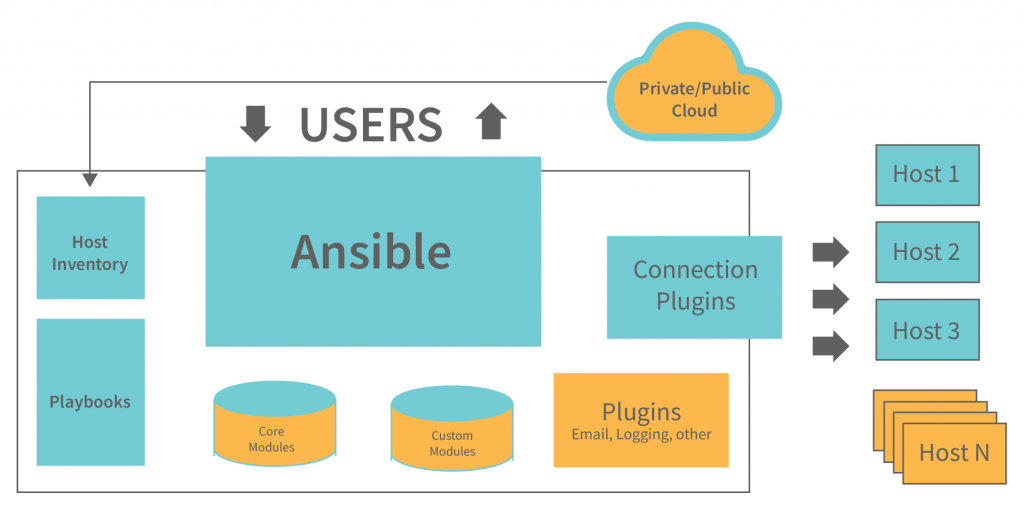
\includegraphics[scale=0.5]{Ansible-Architecture.png}
	\caption{معماری \lr{Ansible}}
	\label{fig: ansible arch}
\end{figure}


\subsubsection{فراهم‌سازی زیرساخت}
فراهم‌سازی زیرساخت فرآیندی است که به راه‌اندازی و پیکربندی اولیه زیرساخت‌های \lr{IT} اختصاص دارد. این فرآیند شامل ایجاد و مدیریت منابعی مانند سرورها، پایگاه داده‌ها، شبکه‌ها و سایر اجزای زیرساختی است. فراهم‌سازی زیرساخت به‌صورت سنتی فرآیندی دستی و زمان‌بر بود، اما با ظهور ابزارهای نوین این فرآیند به‌شدت خودکار و ساده شده است. ابزارهای متن‌بازی مانند \lr{Terraform} برای این کار استفاده می‌شوند. این ابزارها به کاربران امکان می‌دهند تا زیرساخت‌های خود را به‌صورت کد\footnote{\lr{Infrastructure as Code}} تعریف کنند \cite{DevopsIaac1}. این رویکرد به ایجاد و مدیریت منابع زیرساختی به‌صورت قابل تکرار و پایدار کمک می‌کند. \lr{Terraform}، یکی از پرکاربردترین ابزارهای فراهم‌سازی زیرساخت، از زبان \lr{HCL} برای تعریف زیرساخت‌ها استفاده می‌کند. یکی از ویژگی‌های برجسته \lr{Terraform} مدیریت وابستگی‌ها بین منابع است که امکان بازگشت\footnote{\lr{Rollback}} به وضعیت‌های قبلی را نیز فراهم می‌کند \cite{Terraform}. از این ابزارها غالباً برای زیرساخت‌های تغییرناپذیر استفاده می‌شود.

در زیرساخت طراحی‌شده که از \lr{OpenStack} برای ساخت و مدیریت ماشین‌های مجازی استفاده می‌شود، استفاده از \lr{Ansible} به‌عنوان ابزار مدیریت پیکربندی به دلایل متعددی مناسب است. اولاً، \lr{Ansible} با استفاده از \lr{Playbook}های \lr{YAML} امکان خودکارسازی مراحل پیکربندی را فراهم می‌کند، از جمله نصب نرم‌افزارهای مورد نیاز، تنظیمات شبکه و پیکربندی سرویس‌ها. این ویژگی باعث می‌شود که پیکربندی‌ها به‌صورت دقیق و بدون خطا انجام شود. ثانیاً، \lr{Ansible} بدون نیاز به نصب عامل بر روی ماشین‌های مجازی کار می‌کند و از پروتکل \lr{SSH} برای ارتباط استفاده می‌کند که این امر فرآیند پیکربندی را ساده‌تر و سریع‌تر می‌سازد. همچنین، تمامی مراحل پیکربندی به‌صورت کد تعریف می‌شوند که امکان اجرای مجدد و دقیق همان تنظیمات را بر روی ماشین‌های جدید فراهم می‌کند. به‌علاوه، \lr{Ansible} دارای ماژول‌های متعددی برای تعامل با \lr{OpenStack} است که می‌تواند فرآیند ایجاد و مدیریت ماشین‌های مجازی را بهینه‌تر کند. پس از پیکربندی اولیه \lr{VM}ها، \lr{Ansible} می‌تواند خوشه کوبرنتیز را به‌صورت خودکار راه‌اندازی و پیکربندی کند. این شامل نصب ابزارهای مورد نیاز، تنظیمات شبکه و پیکربندی سرویس‌های کوبرنتیز است.

\subsection{خط لوله \lr{CI/CD}}
با افزایش استفاده از سیستم‌های ابری و رویکرد تغییرناپذیر، مفهومی با عنوان \lr{GitOps} معرفی شد که از گیت برای مدیریت زیرساخت و پیکربندی بهره می‌برد. \lr{GitOps} توسط \lr{Weaveworks} در سال ۲۰۱۷ معرفی شد که رویکردی مدرن برای پیاده‌سازی خط لوله \lr{CD} بر روی سیستم‌های ابری است. در حالی که ابزارهای سنتی تحویل مداوم عمدتاً از مدل \lr{Push} استفاده می‌کنند، \lr{GitOps} مدل \lr{Pull} را معرفی می‌کند که به‌خصوص با کانتینرها و پیکربندی‌های اعلامی به‌خوبی کار می‌کند و آن را به یک روند محبوب در اکوسیستم بومی ابر تبدیل کرده است \cite{Devopsgitops}. از معروف‌ترین ابزار کلیدی که فرآیندهای \lr{GitOps} را تسهیل می‌کند می‌توان به \lr{ArgoCD} اشاره کرد.

\begin{figure}[t]
	\centering
	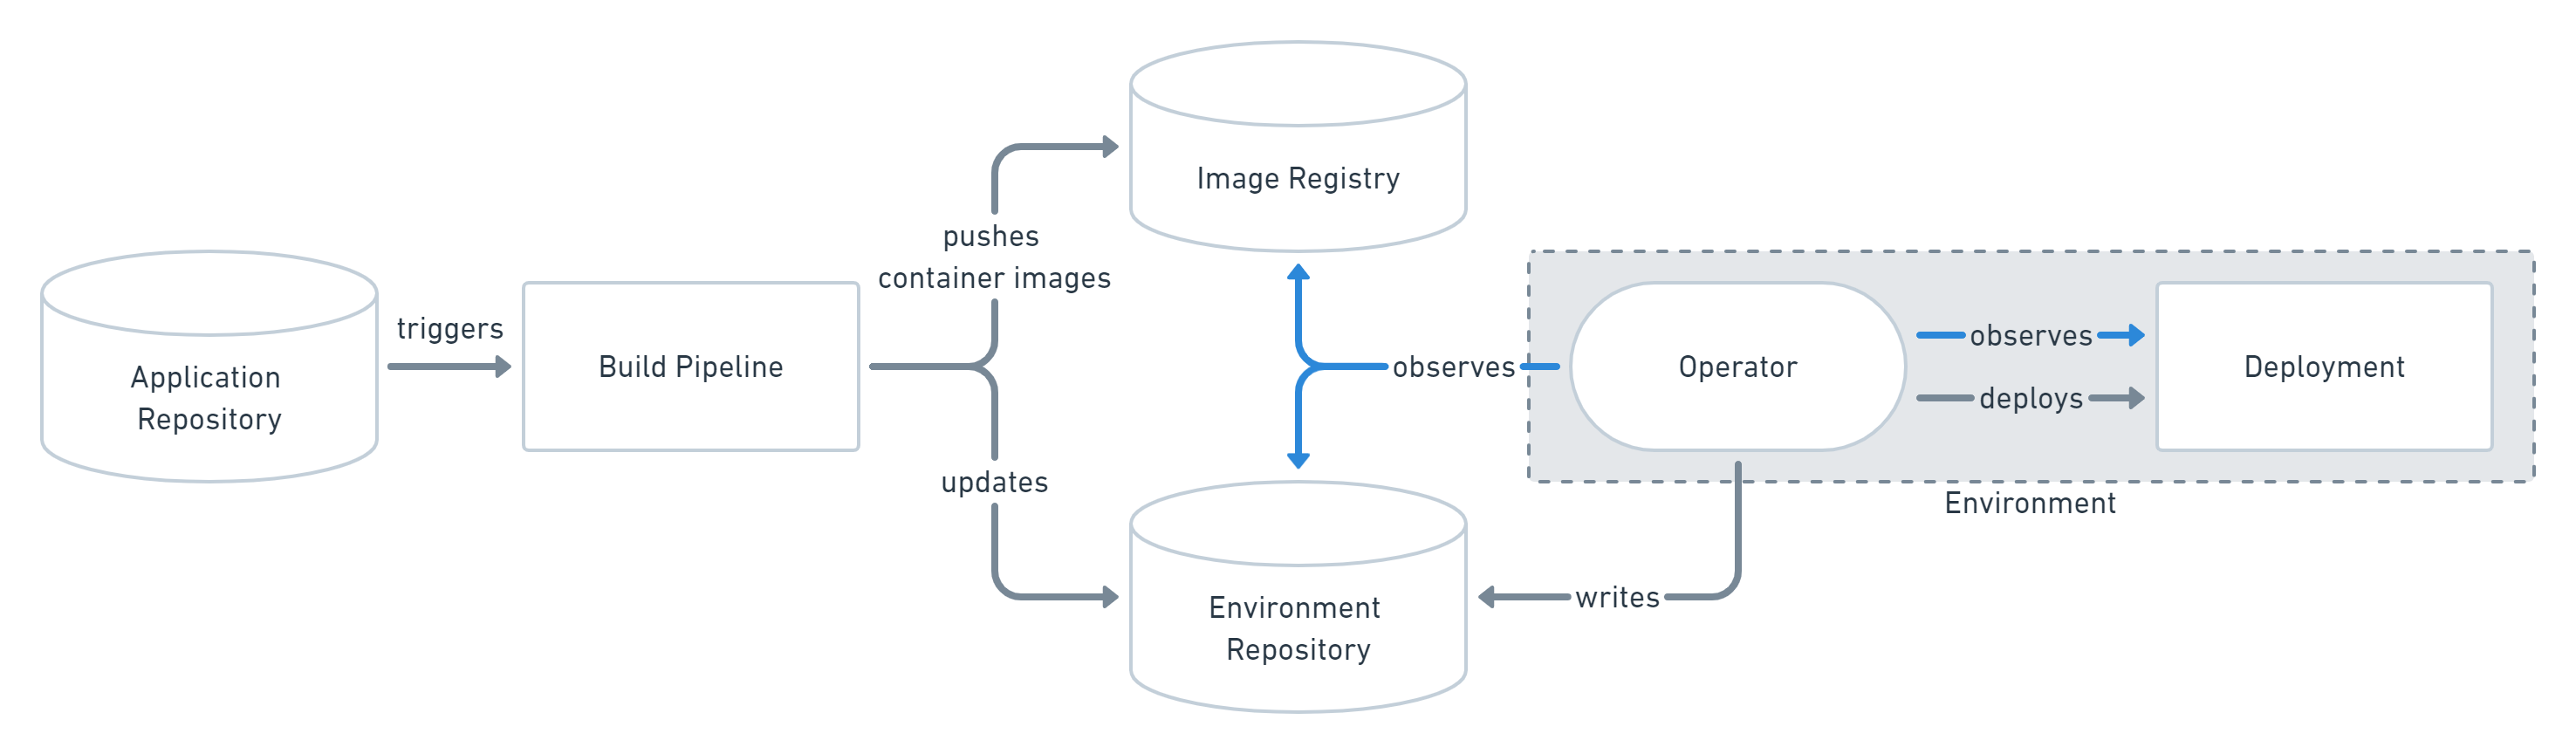
\includegraphics[scale=0.15]{gitops-pull.png}
	\caption{استقرار مبتنی بر \lr{Pull}}
	\label{fig: gitops pull}
\end{figure}

همان‌طور که گفته شد دو رویکرد در پیاده‌سازی خط لوله \lr{CD} وجود دارد. در مدل \lr{Pull} 
(شکل 
~\ref{fig: gitops pull})
مانند \lr{GitOps}، توسعه‌دهندگان حالت مطلوب را در مخزن گیت قرار می‌دهند. ابزاری نظیر \lr{ArgoCD} در محیط تولید به‌صورت خودکار این تغییرات را شناسایی کرده و اعمال می‌کند. این مدل امنیت را افزایش می‌دهد زیرا نیازی به اعتبارنامه‌های دسترسی مستقیم برای توسعه‌دهندگان نیست. همچنین این مدل مشکل استقرارهای مبتنی بر \lr{Push} را حل می‌کند، که در آن محیط تنها زمانی به‌روز می‌شود که مخزن محیط به‌روز شود.
در مقابل، در مدل \lr{Push} (شکل 
~\ref{fig: gitops push})، استقرار در محیط تولید شامل خطوط لوله \lr{CI/CD} با اسکریپت‌هایی است که با هر تغییر در گیت فعال می‌شوند. این اسکریپت‌ها معمولاً ساخت، تست و در نهایت استقرار برنامه‌ها یا تنظیم پیکربندی‌های جدید در محیط تولید را با استفاده از ابزارهای خط فرمان و اعتبارنامه‌های ارائه‌شده انجام می‌دهند. این مدل کنترل دقیق‌تر بر فرآیند استقرار، اعمال سریع تغییرات، انعطاف‌پذیری بالا در مدیریت سناریوهای پیچیده و پشتیبانی بهتر از تغییرات جزئی را فراهم می‌کند، که در محیط‌های متنوع و پویا بسیار مفید است \cite{Devopsgitops}.

\begin{figure}[t]
	\centering
	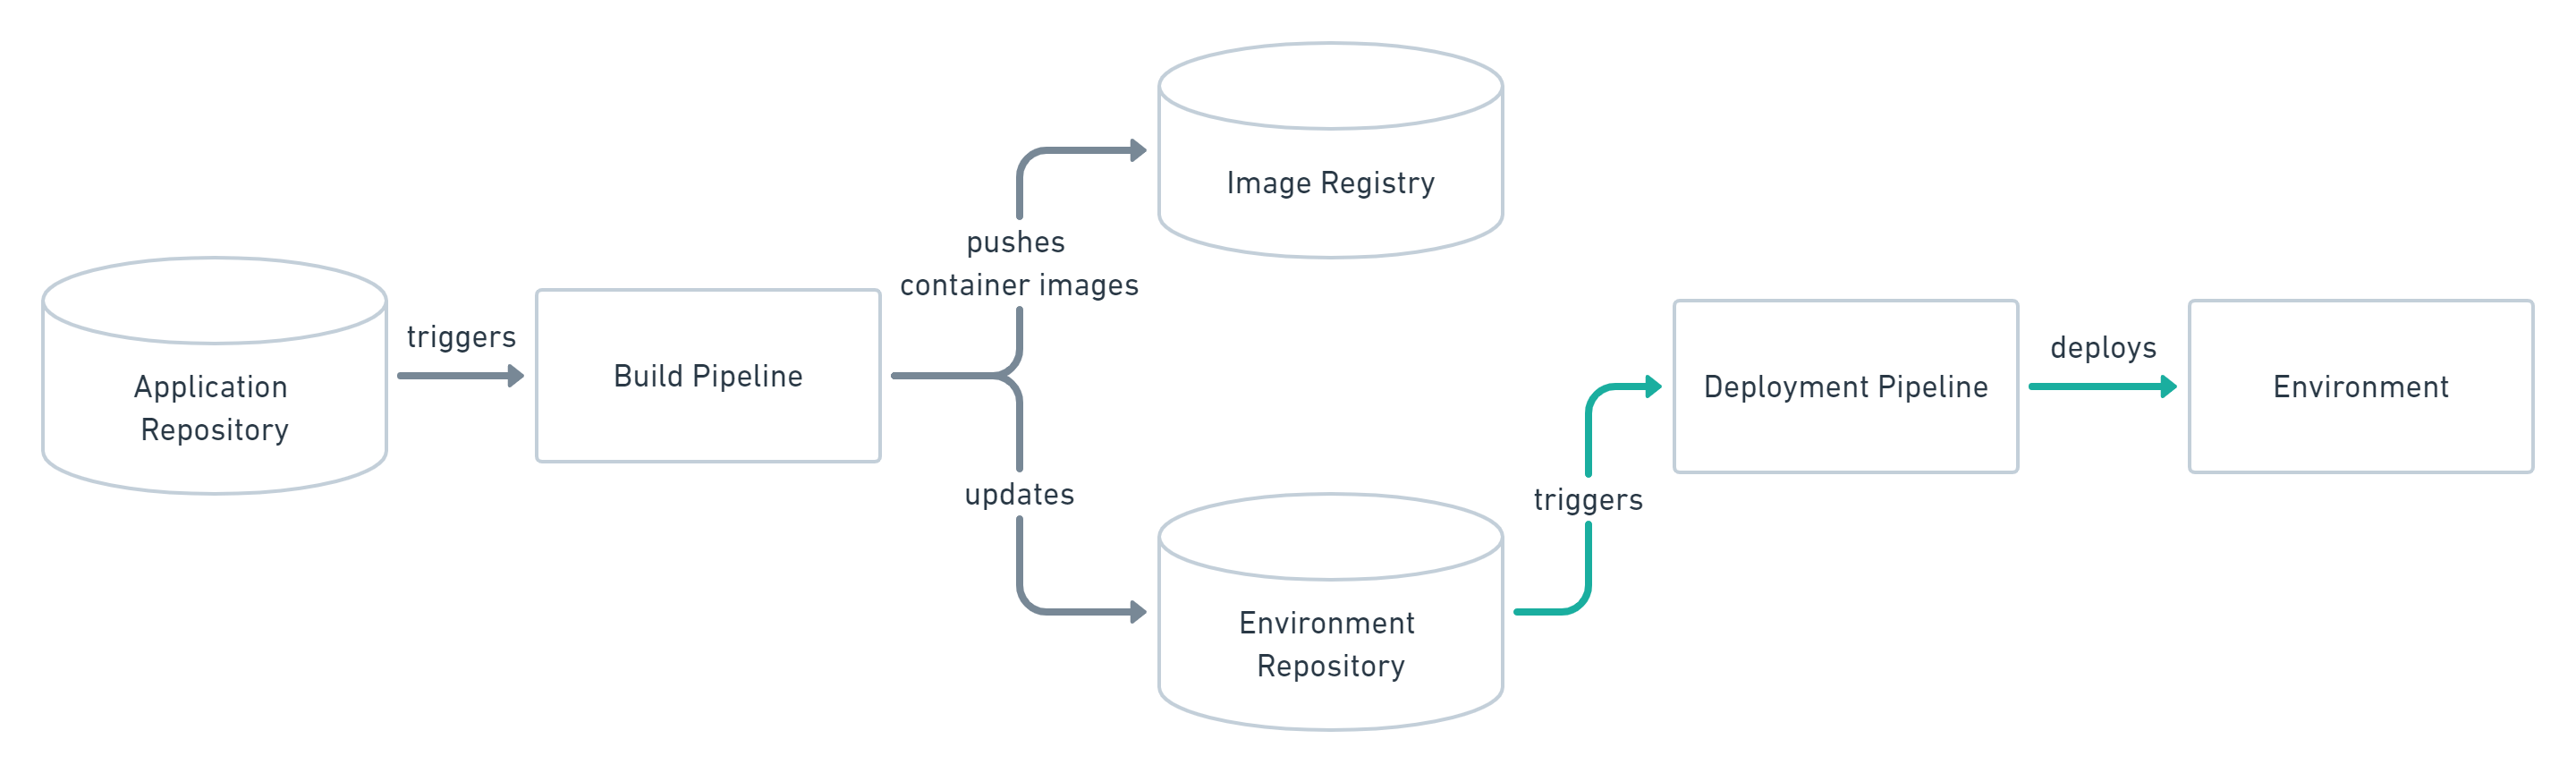
\includegraphics[scale=0.15]{gitops-push.png}
	\caption{استقرار مبتنی بر \lr{Push}}
	\label{fig: gitops push}
\end{figure}

به منظور پیاده‌سازی یک ابزار متن‌باز برای مدیریت خط لوله‌های \lr{CI/CD} که برای سیستم‌های ابری نیز مناسب باشد، رویکرد تغییرپذیر به همراه استراتژی استقرار مبتنی بر \lr{Push} انتخاب شده است. انتخاب رویکرد تغییرپذیر به دلیل نیاز به انعطاف‌پذیری بیشتر در محیط‌هایی که تغییرات مکرر و به‌روزرسانی‌های سریع دارند، انجام شده است. زیرساخت‌های تغییرپذیر به ما امکان می‌دهند تا به‌سرعت به تغییرات نیازمندی‌ها پاسخ دهیم و تنظیمات و پیکربندی‌های جدید را به‌راحتی اعمال کنیم. این ویژگی در محیط‌های توسعه و آزمایش بسیار حیاتی است، زیرا تغییرات مداوم و آزمایش‌های متعدد بخشی از فرآیند توسعه نرم‌افزار هستند. همچنین روش \lr{Push} نیز به دلیل سادگی و کارایی در اعمال به‌روزرسانی‌ها انتخاب شده است. با استفاده از این روش، می‌توانیم به‌روزرسانی‌ها را مستقیماً به سرورها ارسال کنیم و اطمینان حاصل کنیم که تمام سیستم‌ها به‌سرعت و بدون نیاز به مداخله دستی به‌روز می‌شوند. این رویکرد همچنین به کاهش زمان مورد نیاز برای انتشار تغییرات کمک می‌کند. در این راستا، \lr{Jenkins} به‌عنوان ابزار پیاده‌سازی و مدیریت خط لوله \lr{CI/CD} انتخاب شده است. جنکینز به دلیل متن‌باز بودن و دارا بودن تعداد زیادی پلاگین، انعطاف‌پذیری بسیار بالایی دارد و می‌تواند با انواع سیستم‌های ابری و رویکردهای زیرساختی سازگار شود. جنکینز همچنین با \lr{Ansible} که به‌عنوان ابزار مدیریت پیکربندی انتخاب شد، به‌خوبی سازگار است. این ترکیب به ما اجازه می‌دهد تا پیکربندی‌های پیچیده را به‌سادگی مدیریت کنیم و اطمینان حاصل کنیم که تمام زیرساخت‌ها به‌صورت هماهنگ عمل می‌کنند.

\subsection{مخزن کد منبع}

مخزن کد منبع\footnote{\lr{Source Code Repository}} یک سیستم ذخیره‌سازی و مدیریت کد است که به توسعه‌دهندگان این امکان را می‌دهد تا به‌صورت مشترک و هماهنگ بر روی پروژه‌های نرم‌افزاری کار کنند. این مخازن ابزارهای متعددی را برای تسهیل و بهبود فرآیند توسعه نرم‌افزار فراهم می‌کنند. یکی از اصلی‌ترین ویژگی‌های مخزن کد منبع، کنترل نسخه است که به توسعه‌دهندگان این امکان را می‌دهد تا تغییرات کد را پیگیری کرده و به نسخه‌های قبلی بازگردند. این ابزارها با ثبت تاریخچه تغییرات و شاخه‌بندی، امکان مدیریت هم‌زمان چندین ویژگی یا رفع اشکال را فراهم می‌کنند بدون اینکه تغییرات یکدیگر را تحت تأثیر قرار دهند.

رایج‌ترین و پرکاربردترین این مخازن، گیت است که با ابزارهای مختلفی مانند \lr{GitHub}، \lr{GitLab} و \lr{Bitbucket} یکپارچه می‌شود. ازآنجاکه یکی از شرط‌های پیاده‌سازی پلتفرم، متن‌باز بودن ابزارهای آن می‌باشد، \lr{GitLab} برای مدیریت مخزن کد منبع استفاده شده است. در این طراحی \lr{Jenkins} به \lr{GitLab} به‌عنوان مخزن کد متصل شده و هر تغییر در کد منبع باعث اجرا شدن یک خط لوله \lr{CI/CD} مشخص توسط \lr{Jenkins} می‌گردد.


\subsection{مخزن مؤلفه‌ها}
یک مخزن مؤلفه\footnote{\lr{Artifact Repository}} یک سیستم متمرکز برای ذخیره‌سازی، مدیریت و انتشار مؤلفه‌های نرم‌افزاری است. این مؤلفه‌ها شامل هر نوع فایل باینری، کتابخانه، ماژول، پکیج، پلاگین یا حتی مستنداتی می‌شود که در طول چرخه عمر توسعه نرم‌افزار تولید می‌شود. هدف اصلی این مخازن این است که به تیم‌های توسعه اجازه دهند تا به‌راحتی نسخه‌های مختلفی از مؤلفه‌ها را مدیریت و به اشتراک بگذارند، فرآیندهای ساخت و انتشار را ساده کنند و وابستگی‌ها را طور مؤثرتری مدیریت کنند. همچنین، از انتشار مؤلفه‌هایی که هنوز تست نشده‌اند یا از نظر امنیتی مشکلاتی دارند جلوگیری می‌کنند. 
یکی از ابزارهای محبوب و متن‌باز برای مدیریت مخازن مؤلفه‌ها، \lr{Nexus} است. \lr{Nexus} از فرمت‌های مختلف مؤلفه‌ها مانند \lr{Helm}، \lr{apt}، \lr{PyPI} و \lr{Docker} پشتیبانی می‌کند، که این امر آن را به یک ابزار چندمنظوره برای انواع پروژه‌های نرم‌افزاری تبدیل می‌کند. مخازن مؤلفه موردنیاز برای پیاده‌سازی پلتفرم در 4 فرمت \lr{raw}، \lr{apt}، \lr{PyPI} و \lr{Docker} می‌باشد.

\subsubsection{مخازن \lr{APT}}
یک سیستم مدیریت بسته در سیستم‌عامل‌های مبتنی بر دبیان است که به کاربران اجازه می‌دهد تا بسته‌های نرم‌افزاری را به‌راحتی نصب، به‌روزرسانی و حذف کنند. ازآنجاکه بسته‌های استفاده‌شده در سرورها غالباً یکسان می‌باشد، به منظور افزایش سرعت پیاده‌سازی و اعمال تغییرات و پیکربندی تمامی بسته‌های مورد استفاده و نصب‌نشده در محیط، در \lr{Nexus} ذخیره خواهند شد. این امر با استفاده از مخازنی از نوع \lr{Proxy} انجام خواهد شد. در پیاده‌سازی سیستم علاوه بر بسته‌های موجود در \lr{APT} رسمی \lr{Ubuntu}، از مخازن \lr{Containerd} و \lr{Kubernetes} نیز برای نصب و پیاده‌سازی کوبرنتیز نیز استفاده شده است. علاوه بر این، یک مخزن هم برای نصب \lr{Nvidia Driver} و \lr{Nvidida CUDA Toolkit} برای استفاده از واحد پردازنده گرافیکی ایجاد خواهد شد.
\subsubsection{مخزن \lr{PyPI}}
یک مخزن عمومی برای بسته‌های نرم‌افزاری پایتون است که به توسعه‌دهندگان اجازه می‌دهد تا کتابخانه‌ها و ابزارهای خود را منتشر، به‌روزرسانی و مدیریت کنند. کاربران می‌توانند این بسته‌ها را به‌راحتی با استفاده از ابزار \lr{pip} نصب کنند. همانند \lr{APT}، به منظور ذخیره‌سازی تمامی بسته‌های استفاده‌شده در محیط تولید ساخته شده‌اند. این امر باعث افزایش سرعت در نصب مجدد بسته‌ها و پایداری سیستم در زمان‌های قطعی یا خرابی مخازن رسمی می‌شود.
\subsubsection{مخزن \lr{Docker}}
یک سرویس برای \lr{Docker Images} است که به توسعه‌دهندگان اجازه می‌دهد تا تصاویر خود را ذخیره، مدیریت و به اشتراک بگذارند. با توجه به تحریم استفاده از \lr{DockerHub} در ایران و همچنین کند بودن راه‌های جایگزین در گرفتن تصاویر موردنظر از مخازن رسمی این مخزن به وجود آمده که به مخزن رسمی \lr{docker.io} پراکسی شده است. علاوه بر این تصاویر لازم برای پیاده‌سازی و پیکربندی محیط که با خط لوله \lr{CI/CD} ساخته شده‌اند نیز برای استفاده مجدد در این مخازن قرار می‌گیرند.
\subsubsection{مخزن \lr{raw}}
برای ذخیره‌سازی و مدیریت فایل‌ها و داده‌هایی استفاده می‌شود که فرمت خاصی ندارند. این نوع مخزن به توسعه‌دهندگان اجازه می‌دهد تا انواع مختلف فایل‌ها، مانند اسکریپت‌ها، تصاویر، و مستندات را بدون نیاز به ساختاردهی خاصی نگهداری کنند.


\section{معماری خوشه کوبرنتیز}
در طراحی یک پلتفرم \lr{MLOps} جامع و کارآمد که تمامی ابزارهای مورد نیاز را در بر می‌گیرد، هدف اصلی ایجاد یک بستر یکپارچه، مقیاس‌پذیر و انعطاف‌پذیر برای مدیریت چرخه حیات مدل‌های یادگیری ماشین است. این پلتفرم شامل مجموعه‌ای از ابزارها و تکنولوژی‌های متن‌باز است که همگی روی خوشه کوبرنتیز مستقر می‌شوند. استفاده از کوبرنتیز در پلتفرم‌های \lr{MLOps} به دلیل قابلیت‌های منحصربه‌فرد آن در مقیاس‌پذیری و مدیریت خودکار منابع است. کوبرنتیز امکان استقرار مدل‌های یادگیری ماشین در کانتینرها را به‌صورت پویا و قابل‌اطمینان فراهم می‌کند، که این امر منجر به بهبود فرایندهای استقرار و به‌روزرسانی مدل‌ها می‌شود. همچنین، کوبرنتیز با ارائه قابلیت‌های مانیتورینگ و لاگینگ پیشرفته، به تشخیص و رفع سریع مشکلات کمک می‌کند و با ابزارهایی مانند \lr{Kubeflow}، مدیریت چرخه عمر مدل‌ها را تسهیل می‌کند. در ادامه، با الهام از اصول، اجزا و معماری جامع بیان‌شده در فصل سوم، معماری اصلی پلتفرم \lr{MLOps} را که شامل تمام ابزارهایی که بر روی خوشه کوبرنتیز پیاده‌سازی می‌شوند، طراحی کرده و برای هر بخش یک ابزار مناسب معرفی می‌کنیم.


\subsection{مدیریت داده و مدل}
داده‌ها در پلتفرم \lr{MLOps} نقش مهمی دارند. دانشمندان داده به منظور پیاده‌سازی یک مدل یادگیری ماشین نیاز به آموزش این مدل‌ها با استفاده از داده‌های از پیش آماده دارند. این داده‌ها می‌تواند به‌صورت متن، تصویر یا صوت باشد. لذا وجود یک محل ذخیره‌سازی داده برای نگه‌داری داده‌ها در این پلتفرم اساسی است. در کوبرنتیز، چندین روش و نوع ذخیره‌سازی داده وجود دارد که یکی از مهم‌ترین آن‌ها \lr{PVC} می‌باشد که از \lr{PV} برای ذخیره‌سازی داده‌ها استفاده می‌کند.
 
\subsubsection{حجم پایدار و فراهم‌سازهای پویا}
در کوبرنتیز \lr{PV} به‌عنوان منابع ذخیره‌سازی مستقل از چرخه حیات پادها عمل می‌کنند، به این معنا که داده‌ها پس از حذف یا بازسازی پادها همچنان حفظ می‌شوند. \lr{PV}ها توسط مدیر خوشه به‌صورت ایستا یا پویا ایجاد می‌شوند و می‌توانند به \lr{PVC} متصل شوند. \lr{PVC} یک درخواست برای ذخیره‌سازی است که توسط کاربران ایجاد می‌شود و پس از تخصیص، به یک \lr{PV} مرتبط می‌شود. این مکانیزم باعث می‌شود که مدیریت ذخیره‌سازی در خوشه کوبرنتیز ساده‌تر و کارآمدتر شود. \lr{PV}ها می‌توانند از انواع مختلف ذخیره‌سازی مانند دیسک‌های محلی، شبکه‌های ذخیره‌سازی\footnote{\lr{Network File System}} یا راه‌حل‌های ابری استفاده کنند. به علاوه، استفاده از \lr{PV} و \lr{PVC} امکان استفاده مجدد از منابع ذخیره‌سازی را بدون نیاز به تنظیمات دستی پیچیده، برای پادهای مختلف فراهم می‌کند \cite{Kubernetes1, Kubernetes2}.

یکی از قابلیت‌های مهم کوبرنتیز، فراهم‌سازی پویا\footnote{\lr{Dynamic Provisioning}} است که به‌طور خودکار \lr{PV}ها را براساس نیازهای \lr{PVC}ها و کلاس‌های ذخیره‌سازی\footnote{\lr{Storage Class}} ایجاد می‌کند. این ویژگی، نیاز به ایجاد و مدیریت دستی \lr{PV} را توسط مدیران خوشه از بین می‌برد و مدیریت ذخیره‌سازی را ساده‌تر می‌کند. با تعریف کلاس‌های ذخیره‌سازی، می‌توان انواع مختلفی از ذخیره‌سازی را با ویژگی‌های مورد نظر فراهم کرد. هنگامی که یک درخواست ذخیره‌سازی \lr{PVC} با کلاس ذخیره‌سازی مشخص ایجاد می‌شود، کوبرنتیز به‌طور خودکار یک \lr{PV} که متناسب با درخواست است را ایجاد و به درخواست متصل می‌کند \cite{Kubernetes1}. این فرآیند خودکار، نه‌تنها کارایی و بهره‌وری را افزایش می‌دهد بلکه اطمینان می‌دهد که منابع ذخیره‌سازی به‌صورت بهینه و کارآمد تخصیص داده می‌شوند. ابزار متن‌بازی که در این پلتفرم برای مدیریت و ساخت \lr{PV}ها استفاده شده است، \lr{OpenEBS} می‌باشد. با استفاده از این ابزار ما \lr{PV}های مورد نیاز برای ذخیره‌سازی داده‌های پایگاه داده و ذخیره‌سازی شیء مانند \lr{MinIO} را ایجاد می‌کنیم.


\begin{figure}[t]
	\centering
	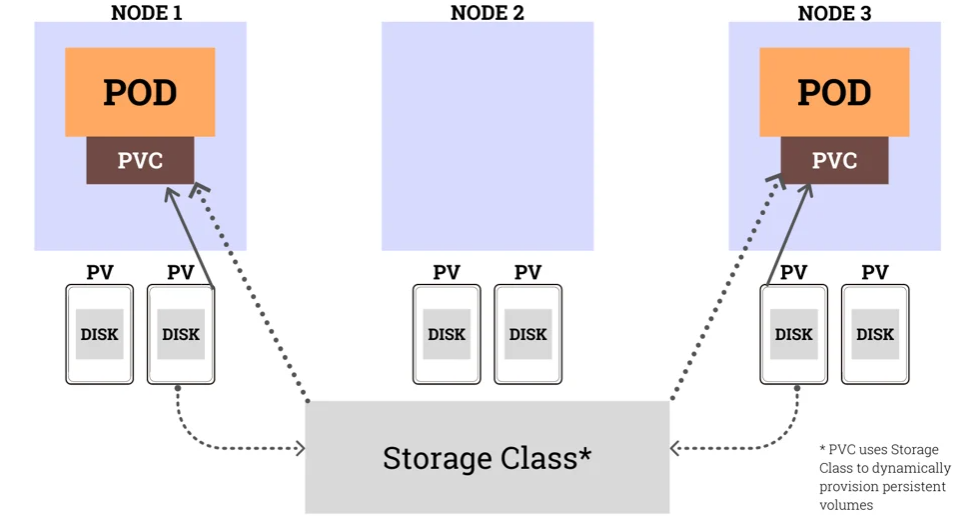
\includegraphics[scale=0.5]{pv-pvc.png}
	\caption{نحوه کار \lr{PV} و \lr{PVC} در خوشه کوبرنتیز}
	\label{fig: pv pvc}
\end{figure}

\subsubsection{ذخیره سازی داده}
برای پلتفرم‌های \lr{MLOps} که نیاز به ذخیره‌سازی حجم زیادی از داده‌ها دارند، استفاده از فضای ذخیره‌سازی ضروری است. ذخیره‌سازی شیء\footnote{\lr{Object Storage}} یک مدل ذخیره‌سازی داده‌ است که برای مدیریت و دسترسی به داده‌های بدون ساختار مانند فایل‌های متنی، تصویری و صوتی استفاده می‌شود. در این مدل، داده‌ها به‌عنوان اشیاء با شناسه منحصربه‌فرد به همراه فراداده‌ها ذخیره می‌شوند. مزایای اصلی ذخیره‌سازی شیء شامل مقیاس‌پذیری بالا، هزینه کمتر و انعطاف‌پذیری در مدیریت داده‌ها است. این سیستم‌ها به‌راحتی می‌توانند به میلیاردها شیء افزایش یابند و برای استفاده در محیط‌های ابری، پشتیبان‌گیری و آرشیو داده‌ها مناسب هستند. همچنین، مدیریت ساده‌تر فراداده‌ها امکان جستجو و دسترسی سریع‌تر به داده‌ها را فراهم می‌کند. \lr{MinIO} \cite{MinIO} یک نرم‌افزار متن‌باز است که به‌منظور ارائه‌ی سرویس ذخیره‌سازی داده طراحی شده است. این نرم‌افزار به دلیل عملکرد بالا و پایداری که دارد، در محیط‌های مختلف از جمله سیستم‌های ابری به‌کار گرفته می‌شود. \lr{MinIO} به‌عنوان جایگزینی برای \lr{Amazon S3} مطرح شده و سازگاری کامل با \lr{API}های \lr{S3} را داراست، که این امر مهاجرت بین این دو سیستم را تسهیل می‌کند.

معماری \lr{MinIO} به‌صورت توزیع‌شده طراحی شده است که این امکان را فراهم می‌کند تا داده‌ها به‌صورت افقی مقیاس‌پذیر باشند. این معماری به‌گونه‌ای است که می‌توان با اضافه کردن گره‌های جدید به خوشه، ظرفیت و عملکرد سیستم را به‌سادگی افزایش داد. در خوشه \lr{MinIO}، داده‌ها به‌صورت خودکار توزیع و تکرار\footnote{\lr{Replication}} می‌شوند تا از دسترس‌پذیری بالا و تحمل خطا اطمینان حاصل شود. یکی از مهم‌ترین تکنیک‌هایی که \lr{MinIO} برای ذخیره‌سازی داده‌ها به‌کار می‌گیرد، کدگذاری پاکسازی\footnote{\lr{Erasure Coding}} است. این تکنیک به \lr{MinIO} اجازه می‌دهد تا داده‌ها را به بلوک‌های کوچک‌تر تقسیم کرده و آن‌ها را به‌صورت توزیع‌شده در چندین گره ذخیره کند. در صورت خرابی یک یا چند گره، \lr{MinIO} می‌تواند داده‌ها را از بلوک‌های باقی‌مانده بازیابی کند، بدون اینکه داده‌ای از دست برود. این روش نه‌تنها فضای ذخیره‌سازی را بهینه می‌کند بلکه تحمل خطای سیستم را نیز افزایش می‌دهد. این ویژگی‌ها \lr{MinIO} را به انتخابی مناسب برای ذخیره‌سازی داده‌های حجیم و پشتیبان‌گیری از آن تبدیل کرده‌اند. در کنار این‌ها یکی از ویژگی‌های مهم \lr{MinIO}، سادگی و کاربرپسندی آن است. نصب و راه‌اندازی این نرم‌افزار بسیار ساده بوده و با چند فرمان ساده قابل انجام است. رابط کاربری وب و خط فرمان (\lr{mc}) نیز به کاربران اجازه می‌دهند تا مدیریت و مانیتورینگ سرورها و داده‌ها را به‌سادگی انجام دهند.

\begin{figure}[t]
	\centering
	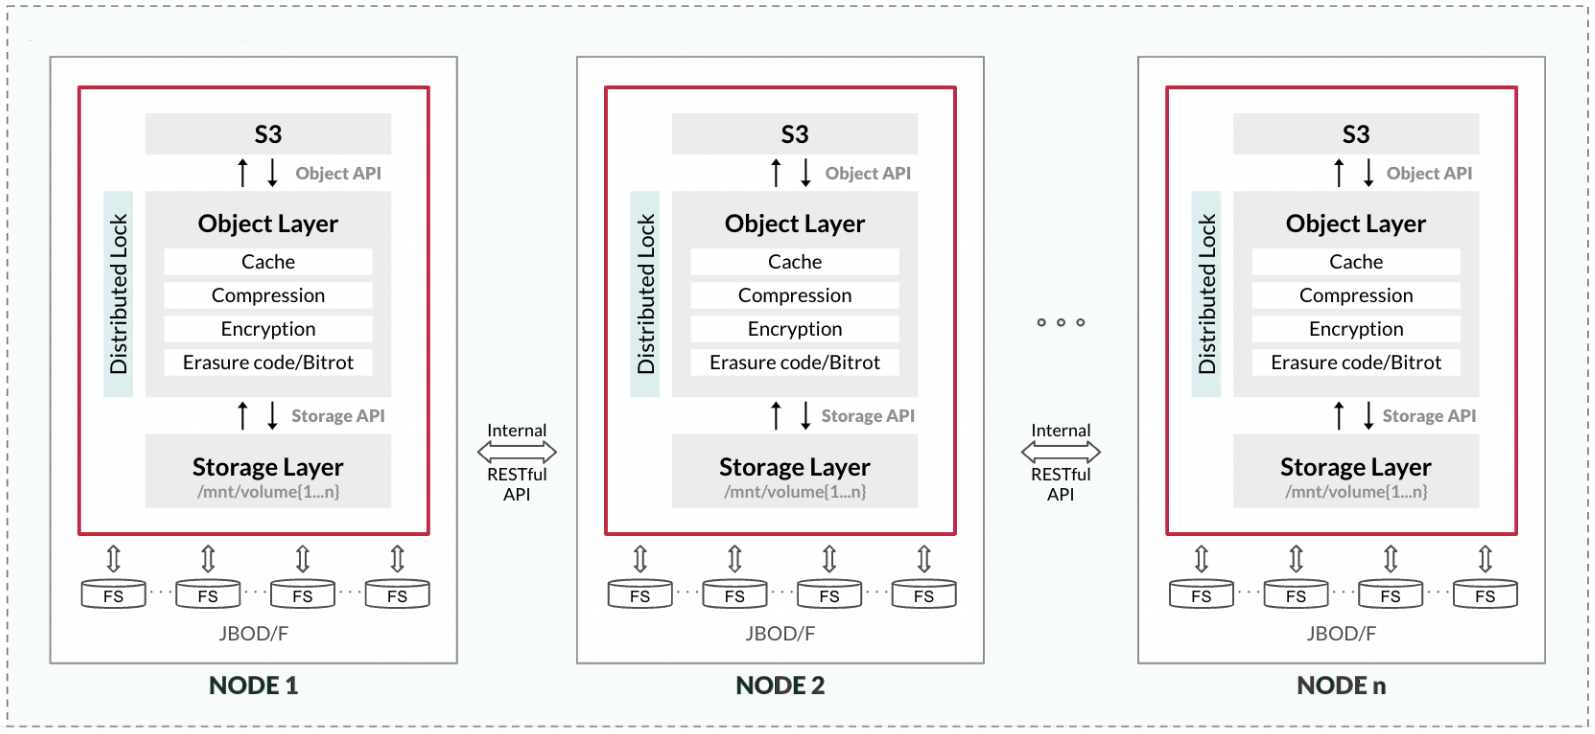
\includegraphics[scale=0.8]{minio-arch.png}
	\caption{معماری \lr{MinIO}}
	\label{fig: minio arch}
\end{figure}

در معماری طراحی‌شده برای این پلتفرم، داده‌ها ابتدا در \lr{MinIO} و در باکت‌های مجزا ذخیره می‌شوند. دانشمندان داده به همراه مهندسان داده با استفاده از کتابخانه‌های پایتون از این داده‌ها استفاده کرده و پیش‌پردازش‌های موردنظر را روی داده‌ها انجام داده و ویژگی‌های موردنظر را استخراج می‌کنند. در نهایت این ویژگی‌ها را می‌توانند در همان \lr{MinIO} و یا در پایگاه‌داده‌هایی که به همین منظور طراحی شده ذخیره نمایند.


\subsubsection{پایگاه داده}
به‌منظور ذخیره‌سازی داده‌های ساختاریافته\footnote{\lr{Structured}} مانند داده‌های جدولی و یا ویژگی‌های به‌دست‌آمده در خط لوله مهندسی ویژگی می‌توان از پایگاه‌های داده استفاده نمود. در این راستا، از \lr{PostgreSQL} و \lr{Redis} به‌عنوان انباره‌های داده آنلاین و آفلاین استفاده شده است.

\lr{PostgreSQL}
به‌عنوان انباره داده آفلاین مورد استفاده قرار می‌گیرد. این سیستم مدیریت پایگاه داده رابطه‌ای، به دلیل پشتیبانی از تراکنش‌های \lr{ACID}، قابلیت اطمینان بالا و توانایی پشتیبانی از انواع داده‌های پیچیده، انتخاب مناسبی برای ذخیره‌سازی داده‌های آموزشی و ویژگی‌های به‌دست‌آمده از آن، لاگ‌ها و اطلاعات تحلیلی است. \lr{PostgreSQL} با قابلیت‌های تحلیلی قوی و مقیاس‌پذیری مناسب، امکان تجزیه‌وتحلیل عمیق داده‌ها و مدیریت متاداده‌های مدل‌ها را فراهم می‌کند.

در مقابل، \lr{Redis} یک انباره داده در حافظه\footnote{\lr{In-memory}} است که برای کاربردهای آنلاین در معماری \lr{MLOps} بسیار مناسب است. \lr{Redis} به دلیل سرعت بالای خواندن و نوشتن داده‌ها و پشتیبانی از ساختارهای داده متنوع، برای ذخیره‌سازی نتایج پیش‌بینی مدل‌ها، کش کردن داده‌های موقت و مدیریت صف‌ها و تراکنش‌های سریع استفاده می‌شود. این امر به بهبود کارایی و کاهش زمان پاسخ‌دهی سیستم کمک می‌کند.

ترکیب \lr{PostgreSQL} و \lr{Redis} در این معماری، یک راهکار جامع و کارآمد برای مدیریت داده‌ها فراهم می‌کند. \lr{PostgreSQL} با امکانات پیشرفته‌اش به‌عنوان انباره داده آفلاین، و \lr{Redis} با سرعت بالایش به‌عنوان انباره داده آنلاین می‌تواند نیازهای مختلف سیستم را فراهم سازد.


\subsubsection{بانک مدل و انبار فراداده}
بانک مدل یکی از ابزارهای بسیار مهم در مدیریت مدل‌های یادگیری ماشین است که به تیم‌ها کمک می‌کند تا مدل‌های خود را به‌صورت سازمان‌یافته ذخیره، مدیریت و ردیابی کنند. همچنین اطلاعات مربوط به هر مدل را از جمله نسخه، تاریخ آخرین آموزش، معیارهای ارزیابی و مستندات مربوطه را نگهداری می‌کند. این امر به تیم‌ها کمک می‌کند تا با استفاده از نسخه‌های مختلف مدل‌ها، آزمایش‌های مختلفی انجام دهند و بهترین مدل را انتخاب کنند. همچنین به هنگام بروز مشکل در مدل‌های جدید، می‌توان از مدل‌های قابل‌قبول قبلی برای محیط عملیاتی استفاده کرد. انبار فراداده یادگیری ماشین نیز برای پیگیری و ذخیره‌سازی اطلاعات مربوط به هر مرحله از جریان کاری یادگیری ماشین استفاده می‌شوند. فراداده‌ها می‌توانند شامل جزئیاتی نظیر تاریخ و زمان آموزش مدل، مدت‌زمان هر مرحله از آموزش، پارامترهای استفاده‌شده، معیارهای عملکرد مدل و سلسله‌مراتب مدل (مثل داده‌ها و کدهای استفاده‌شده) باشند.

از ابزارهای معروف متن‌باز در این بخش می‌توان به \lr{MLflow} اشاره کرد. \lr{MLflow} یک پلتفرم مدیریت چرخه عمر یادگیری ماشین است که توسط \lr{Databricks} توسعه داده شده است. این ابزار به تیم‌های یادگیری ماشین کمک می‌کند تا فرآیند توسعه، آزمایش و مدیریت مدل‌های خود را بهبود بخشند. این ابزار شامل چهار جزء اصلی است: مدیریت آزمایش\footnote{\lr{Experiment Management}} که امکان ردیابی و مقایسه آزمایش‌های مختلف را فراهم می‌کند، ردیابی\footnote{\lr{Tracking}} که به ثبت و مدیریت پارامترها، معیارهای عملکرد و مدل‌های ساخته‌شده کمک می‌کند، بسته‌بندی\footnote{\lr{Packaging}} که مدل‌های آموزش‌دیده را به‌صورت استاندارد و قابل‌اجرا در محیط‌های مختلف بسته‌بندی و ذخیره‌سازی می‌کند، و استقرار که اجرای مدل‌ها را در محیط‌های مختلف مانند داکر و کوبرنتیز ساده‌تر می‌کند.

با توجه به کاهش پیچیدگی در طراحی می‌توان از ابزارهای استفاده‌شده در بخش‌های دیگر برای پیاده‌سازی این بخش استفاده کرد. ازآنجاکه \lr{MinIO} توانایی ذخیره‌سازی هر مؤلفه‌ای را به همراه فراداده‌های آن دارد، از این ابزار برای \lr{Packaging} استفاده شده است. سایر بخش‌ها نیز به دلیل یکپارچگی با اجزا دیگر در پلتفرم طراحی‌شده با استفاده از \lr{Kubeflow} پیاده‌سازی شده است.

\subsection{شبکه}
بسیاری از برنامه‌های مدرن با استفاده از معماری میکروسرویس توزیع‌شده ساخته می‌شوند که باعث می‌شود هر سرویس ساده و دارای مسئولیت مشخص باشد. هر میکروسرویس \lr{API}های خود را تعریف کرده و سرویس‌ها برای پاسخ‌گویی به درخواست‌های کاربران نهایی از این \lr{API}ها برای تعامل با یکدیگر استفاده می‌کنند. در کوبرنتیز، به‌منظور شبکه‌سازی برای ارتباط بین پادها و سرویس‌ها، به هر پاد یک آدرس \lr{IP} منحصربه‌فرد اختصاص داده می‌شود که این امکان را فراهم می‌کند تا پادها بدون نیاز به \lr{NAT} به‌صورت مستقیم با یکدیگر ارتباط برقرار کنند. با افزایش تعداد این میکروسرویس‌ها، مدیریت ارتباطات، امنیت و پایش این سرویس‌ها به چالشی بزرگ تبدیل می‌شود که می‌توان با \lr{Service Mesh} آن را مدیریت کرد \cite{Istio1}.

سرویس مش یک لایه زیرساختی است که مدیریت ارتباط بین سرویس‌ها در معماری میکروسرویس‌ها را بر عهده دارد. این لایه قابلیت‌هایی مانند مشاهده‌پذیری، مدیریت ترافیک و امنیت را بدون تغییر کدهای برنامه اضافه می‌کند. \lr{Istio} یک سیستم متن‌باز برای مدیریت اتصال، امنیت و مشاهده‌پذیری در معماری‌های میکروسرویس‌ها است که به‌عنوان سرویس مش شناخته می‌شود. این ابزار با افزودن یک لایه مستقل بین میکروسرویس‌ها و شبکه، توانایی‌هایی مانند مسیریابی هوشمند، ترافیک مدیریت‌شده، نظارت و امنیت را بهبود می‌بخشد. این سیستم از پروکسی‌های جانبی\footnote{\lr{Sidecar proxies}} برای کنترل ارتباطات بین میکروسرویس‌ها استفاده می‌کند که این پروکسی‌ها معمولاً از \lr{Envoy}، یک پروکسی سریع و سبک، بهره می‌برند \cite{Istio2}. از ویژگی‌های مهم \lr{Istio} می‌توان به سه مورد زیر اشاره کرد:
\begin{itemize}
	\item 
	مدیریت ترافیک:
	به کاربران اجازه می‌دهد تا ترافیک بین سرویس‌ها را به‌صورت دقیق کنترل و مدیریت کنند. با استفاده از قابلیت‌های مسیریابی پیشرفته، کاربران می‌توانند قوانین پیچیده‌ای برای مسیریابی ترافیک تعریف کنند. این قوانین شامل تقسیم بار\footnote{\lr{Load balancing}}، مسیریابی مبتنی بر نسخه (برای پیاده‌سازی به‌روزرسانی‌های متوالی) و مدیریت ترافیک‌های خطا\footnote{\lr{Fault injection}} می‌شوند. این ویژگی‌ها به توسعه‌دهندگان کمک می‌کنند تا با اطمینان بیشتری به‌روزرسانی‌ها و تغییرات را در سیستم‌های خود اعمال کنند \cite{Istio2}.
	\item 
	امنیت:
	امکانات امنیتی جامعی برای ارتباطات سرویس به سرویس فراهم می‌کند. این امکانات شامل احراز هویت\footnote{\lr{Authentication}} و مجوزدهی\footnote{\lr{Authorization}} مبتنی بر سیاست‌های امنیتی است. \lr{Istio} با استفاده از \lr{MTLS} ارتباطات بین سرویس‌ها را رمزنگاری می‌کند و اطمینان حاصل می‌کند که فقط سرویس‌های معتبر می‌توانند با یکدیگر ارتباط برقرار کنند. این قابلیت‌ها به افزایش امنیت سیستم‌های میکروسرویس کمک شایانی می‌کنند.
	\item
	مشاهده‌پذیری و نظارت:
	قابلیت‌های گسترده‌ای شامل جمع‌آوری و نمایش لاگ‌ها، متریک‌ها و تریس‌ها\footnote{\lr{Trace}} برای مشاهده‌پذیری و نظارت ارتباطات بین سرویس‌ها فراهم می‌کند. با استفاده از ابزارهای یکپارچه‌سازی‌شده مانند \lr{Prometheus} و \lr{Grafana} کاربران می‌توانند به‌صورت جامع عملکرد و سلامت سیستم‌های خود را نظارت کنند.
\end{itemize}

همان‌طور که معماری این سیستم را در شکل 
~\ref{fig: istio arch}
می‌بینید، \lr{Istio} به دو بخش اصلی سطح داده\footnote{\lr{Data plane}} و سطح کنترل\footnote{\lr{Control plane}} تقسیم می‌شود.

\begin{figure}[t]
	\centering
	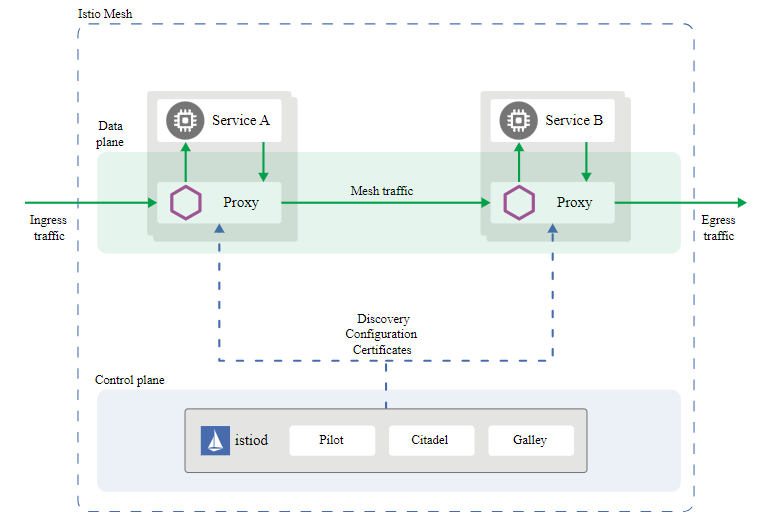
\includegraphics[scale=0.7]{istio.png}
	\caption{معماری \lr{Istio}}
	\label{fig: istio arch}
\end{figure}

\subsubsection{سطح داده}
سطح داده مدیریت ارتباط بین سرویس‌ها را بر عهده دارد. در یک شبکه سنتی بدون سرویس مش، شبکه نمی‌تواند ترافیک را بفهمد و بنابراین نمی‌تواند تصمیمات مبتنی بر نوع ترافیک یا منبع و مقصد آن بگیرد. با استفاده از این سیستم، هر ترافیک شبکه‌ای که از سرویس‌ها خارج یا به آن‌ها وارد می‌شود توسط یک پروکسی رهگیری می‌شود. سطح داده شامل مجموعه‌ای از پروکسی‌های هوشمند به نام \lr{Envoy} است که به‌صورت \lr{Sidecar} به هر سرویس در مش اضافه می‌شوند. این پروکسی‌ها وظیفه میانجی‌گری و کنترل تمامی ارتباطات شبکه‌ای بین میکروسرویس‌ها را بر عهده دارند \cite{Istio2}.

\lr{Envoy}
پراکسی، به‌عنوان یک پروکسی با عملکرد بالا، قابلیت‌های گسترده‌ای را برای مدیریت ترافیک میکروسرویس‌ها در سرویس مش فراهم می‌کند. این قابلیت‌ها شامل کشف سرویس پویا است که به‌طور خودکار سرویس‌ها را شناسایی کرده و به تغییرات در توپولوژی پاسخ می‌دهد. تقسیم بار ترافیک را بهینه‌سازی می‌کند \cite{Istio2}. این ابزار از پروتکل‌های \lr{HTTP/2} و \lr{gRPC} برای بهبود کارایی پشتیبانی می‌کند و با استفاده از قطع‌کننده‌های مدار\footnote{\lr{Circuit Breakers}} از بارگذاری بیش‌ازحد سرویس‌ها جلوگیری می‌کند. این پروکسی همچنین قابلیت بررسی سلامت سرویس‌ها، تزریق خطا برای شبیه‌سازی خرابی‌ها و جمع‌آوری تلمتری غنی را دارد.

\subsubsection{سطح کنترل}
سطح کنترل مسئول مدیریت و پیکربندی پروکسی‌های تشکیل‌دهنده سطح داده است. این سطح، پیکربندی مورد نظر شما را که از طریق سیاست‌ها و قوانین تعریف می‌شود، دریافت می‌کند و با استفاده از دید خود نسبت به سرویس‌ها در داخل مش، پروکسی‌ها را به‌صورت پویا برنامه‌ریزی می‌کند. هنگامی‌که قوانین یا محیط تغییر می‌کنند، سطح کنترل پروکسی‌ها را به‌روزرسانی می‌کند \cite{Istio2}. این پیکربندی پویا به مدیریت ترافیک و سیاست‌ها به‌صورت بلادرنگ این امکان را می‌دهد تا سرویس مش به‌سرعت با تغییرات نیازهای برنامه یا زیرساخت‌ها سازگار شود.

اصلی‌ترین جزء صفحه کنترل \lr{Istiod} نام دارد که مسئول کشف سرویس، مدیریت پیکربندی و مدیریت گواهی‌ها است. این ابزار، قواعد مسیریابی را به پیکربندی‌های \lr{Envoy} تبدیل کرده و به سایدکارها ارسال می‌کند. \lr{Istiod} به‌عنوان مرجع صدور گواهی\footnote{\lr{Certificate Authority}} عمل کرده و ارتباطات امن \lr{MTLS} را در صفحه داده تضمین می‌کند. همچنین، با مدیریت هویت و اعتبارنامه‌ها، احراز هویت قوی و اجرای سیاست‌های امنیتی را فراهم می‌کند.

\subsection{مدیریت کاربران و چندمستاجری}
پشتیبانی از چندین کاربر و چندمستاجری\footnote{\lr{Multi-Tenancy}} در پلتفرم ابری یکی از ویژگی‌های کلیدی است که به کاربران مختلف اجازه می‌دهد به‌صورت امن و مستقل بر روی همان پلتفرم کار کنند. این قابلیت با استفاده از مفاهیم ایزوله‌سازی، احراز هویت و مجوزدهی پیاده‌سازی شده است. در ادامه به جزئیات این فرآیندها می‌پردازیم.

\subsubsection{احراز هویت}
احراز هویت در پلتفرم از طریق ترکیبی از پروتکل \lr{OIDC}\footnote{\lr{OpenID Connect}} و \lr{Istio}، به همراه ابزار \lr{Dex} برای مدیریت هویت\footnote{\lr{Identity Provider}} و یکپارچگی با سیستم‌های احراز هویت خارجی، انجام می‌شود. پروتکل \lr{OIDC} یک لایه احراز هویت بر روی \lr{OAuth 2.0} است که امکان تأیید هویت کاربران و دریافت اطلاعات پروفایل آن‌ها را فراهم می‌کند \cite{OIDC1}. \lr{Dex} نیز یک سرویس منبع باز است که به‌عنوان یک ارائه‌دهنده هویت \lr{OIDC} عمل می‌کند و می‌تواند با سیستم‌های هویتی مختلفی مانند \lr{LDAP} و \lr{Active Directory} یکپارچه شود.

\begin{figure}[t]
	\centering
	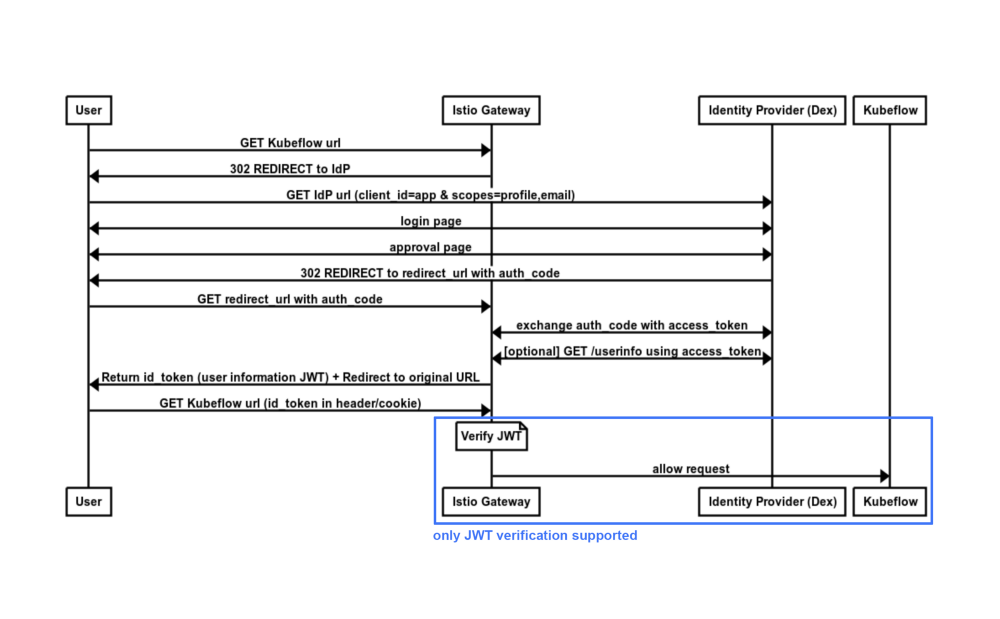
\includegraphics[scale=0.45]{OIDC-dex.png}
	\caption{روند احراز هویت}
	\label{fig: auth flow}
\end{figure}

شکل 
~\ref{fig: auth flow}
روند احراز هویت یک کاربر با استفاده از پروتکل \lr{OIDC} را نشان می‌دهد. کاربران ابتدا به رابط کاربری پلتفرم ابری وارد می‌شوند. در این مرحله، \lr{Dex} به‌عنوان ارائه‌دهنده هویت، صفحه ورود را به کاربر نشان می‌دهد. سپس \lr{Dex} اطلاعات کاربر را از سیستم‌های احراز هویت خارجی می‌گیرد و پس از تأیید هویت، یک توکن \lr{OIDC} صادر می‌کند. پس از احراز هویت موفقیت‌آمیز، توکن \lr{OIDC} به کاربر بازگردانده می‌شود و در هر درخواست \lr{HTTP} به پلتفرم ابری، به‌عنوان هدر \lr{Authorization} ارسال می‌شود \cite{OIDC1}. \lr{Istio} به‌عنوان یک پروکسی معکوس عمل کرده و تمامی درخواست‌های ورودی را بررسی می‌کند. سرویس مش با استفاده از توکن \lr{OIDC} ارسال‌شده توسط کاربر، هویت وی را تأیید می‌کند. پس از تأیید هویت توسط \lr{Istio}، درخواست به سرور \lr{API} پلتفرم ابری ارسال می‌شود. سرور \lr{API} نیز هدرهای مربوط به اطلاعات هویتی را بررسی و پردازش می‌کند.

\subsubsection{ایزوله‌سازی}
ایزوله‌سازی در این پلتفرم با استفاده از \lr{namespace}های کوبرنتیز انجام می‌شود. هر \lr{namespace} به یک یا چند کاربر اختصاص داده می‌شود و منابع هر کاربر مانند خط لوله‌ها و داده‌ها در \lr{namespace} مخصوص به خود قرار می‌گیرند. این روش تضمین می‌کند که کاربران تنها به منابع خود دسترسی دارند و نمی‌توانند به منابع سایر کاربران دسترسی پیدا کنند.

\subsubsection{مجوزدهی}
مجوزدهی در پلتفرم ابری با استفاده از \lr{RBAC}\footnote{\lr{Role-based access control}} کوبرنتیز انجام می‌شود. مجوزها به‌صورت نقش‌ها تعریف‌شده و از طریق \lr{RoleBinding} به کاربران یا گروه‌های کاربران اختصاص داده می‌شوند \cite{Kubernetes1}. این روش به مدیران سیستم اجازه می‌دهد تا دسترسی‌های دقیقی برای کاربران تعیین کنند، مثلاً کاربری تنها بتواند خط لوله‌ها را مشاهده کند اما نتواند آن‌ها را اجرا کند.

\subsection{نظارت}
نظارت در پلتفرم \lr{MLOps} برای اطمینان از عملکرد بهینه و پایداری مدل‌های یادگیری ماشین از اهمیت ویژه‌ای برخوردار است. متریک‌ها در \lr{MLOps} به سه دسته اصلی متریک‌های سیستم، متریک‌های مدل و متریک‌های داده تقسیم می‌شوند.

\subsubsection{متریک‌های سیستم}
متریک‌های سیستم اطلاعاتی درباره مصرف منابع مانند \lr{CPU}، حافظه، استفاده از دیسک و ترافیک شبکه را شامل می‌شوند. این متریک‌ها به شناسایی مشکلات زیرساختی کمک می‌کنند که ممکن است بر عملکرد کلی سیستم تأثیر بگذارند. مثلاً افزایش مصرف \lr{CPU} یا حافظه می‌تواند نشان‌دهنده بار غیرعادی یا مشکلات در کد مدل باشد.

\subsubsection{متریک‌های مدل}
متریک‌های مدل برای ارزیابی عملکرد مدل‌های یادگیری ماشین استفاده می‌شوند و شامل پارامترهایی مانند مدت‌زمان پیش‌بینی، دقت، \lr{F1-score} و نرخ خطا هستند. مدت‌زمان پیش‌بینی نشان‌دهنده مدت‌زمان لازم برای انجام یک پیش‌بینی است و افزایش غیرعادی آن می‌تواند نشان‌دهنده مشکلات کارایی باشد. دقت مدل به ارزیابی کیفیت پیش‌بینی‌ها کمک می‌کند و کاهش در این متریک‌ها ممکن است نشان‌دهنده نیاز به بازآموزی مدل\footnote{\lr{Model Retraining}} باشد. نرخ خطا نیز به شناسایی مشکلات احتمالی در داده‌ها یا الگوریتم‌ها کمک می‌کند.

\subsubsection{متریک‌های داده}
متریک‌های داده شامل کیفیت داده‌ها، تغییرات در توزیع داده‌ها\footnote{\lr{Data Drift}} و نرخ داده‌های مفقود می‌باشند. این متریک‌ها برای تضمین کیفیت داده‌های ورودی و جلوگیری از بروز مشکلات ناشی از داده‌های نادرست یا ناکافی ضروری هستند. مثلاً تغییرات ناگهانی در توزیع داده‌ها می‌تواند نشان‌دهنده تغییرات در رفتار کاربران یا نقص در فرآیند جمع‌آوری داده‌ها باشد. نرخ داده‌های مفقود نیز به شناسایی مشکلات در جریان داده‌ها کمک می‌کند و از تأثیرگذاری منفی بر عملکرد مدل جلوگیری می‌کند.

یکی از ابزارهای کلیدی برای جمع‌آوری این متریک‌ها \lr{Prometheus} است که برای جمع‌آوری، ذخیره‌سازی و مدیریت متریک‌ها به کار می‌رود. \lr{Prometheus} از یک مدل داده مبتنی بر سری‌های زمانی و یک زبان پرس‌وجوی قدرتمند به نام \lr{PromQL} استفاده می‌کند. \lr{Prometheus} متریک‌ها را از طریق \lr{scraping} از \lr{endpoint}های مشخص‌شده جمع‌آوری می‌کند. این \lr{endpoint}ها می‌توانند توسط سرویس‌ها، اپلیکیشن‌ها و مدل‌های مختلف ارائه شوند که در آن‌ها متریک‌های مختلف به‌صورت فرمت‌های مشخص مانند \lr{JSON} قرار دارند. هر متریک می‌تواند دارای چندین برچسب باشد که به فیلتر کردن و گروه‌بندی داده‌ها کمک می‌کند. این برچسب‌ها می‌توانند شامل نام سرویس، نسخه مدل، نام مدل و دیگر اطلاعات مرتبط باشند \cite{Prometheus1}.

برای جمع‌آوری متریک‌ها، \lr{Prometheus} به‌طور دوره‌ای به \lr{endpoint}های مشخص‌شده مراجعه کرده و داده‌ها را دریافت می‌کند. این داده‌ها سپس در یک پایگاه داده زمان-سری ذخیره می‌شوند که امکان اجرای پرس‌وجوهای پیچیده و ایجاد هشدارهای مختلف را فراهم می‌کند. با تعریف آستانه‌های مختلف، \lr{Prometheus} می‌تواند در صورت بروز شرایط بحرانی مانند افزایش غیرعادی زمان پیش‌بینی یا مصرف بیش‌ازحد منابع، به تیم‌ها هشدار دهد \cite{Prometheus1}. از \lr{Alertmanager} نیز در کنار \lr{Prometheus} برای مدیریت هشدارها استفاده می‌شود. هنگامی‌که یک قانون هشدار در \lr{Prometheus} فعال می‌شود، هشدار به \lr{Alertmanager} ارسال می‌شود. \lr{Alertmanager} بر اساس پیکربندی‌های تعریف‌شده، هشدار را به گیرندگان مناسب ارسال می‌کند. این گیرندگان می‌توانند شامل ایمیل‌ها، سرویس‌های پیام‌رسانی (مانند \lr{Slack}) و یا حتی \lr{runbooks}‌ها برای اجرای خودکار اقدامات باشند. درنهایت، با استفاده از داشبوردهای تعاملی و قابل سفارشی‌سازی \lr{Grafana}، تیم‌ها می‌توانند متریک‌های جمع‌آوری‌شده توسط \lr{Prometheus} را به‌صورت بصری مشاهده و تحلیل کنند و با استفاده از فیلترهای مختلف، تحلیل‌های دقیقی از عملکرد مدل‌ها و سیستم‌ها ارائه دهند \cite{Grafana} (شکل ~\ref{fig: monitoring arch}).

\begin{figure}[!t]
	\centering
	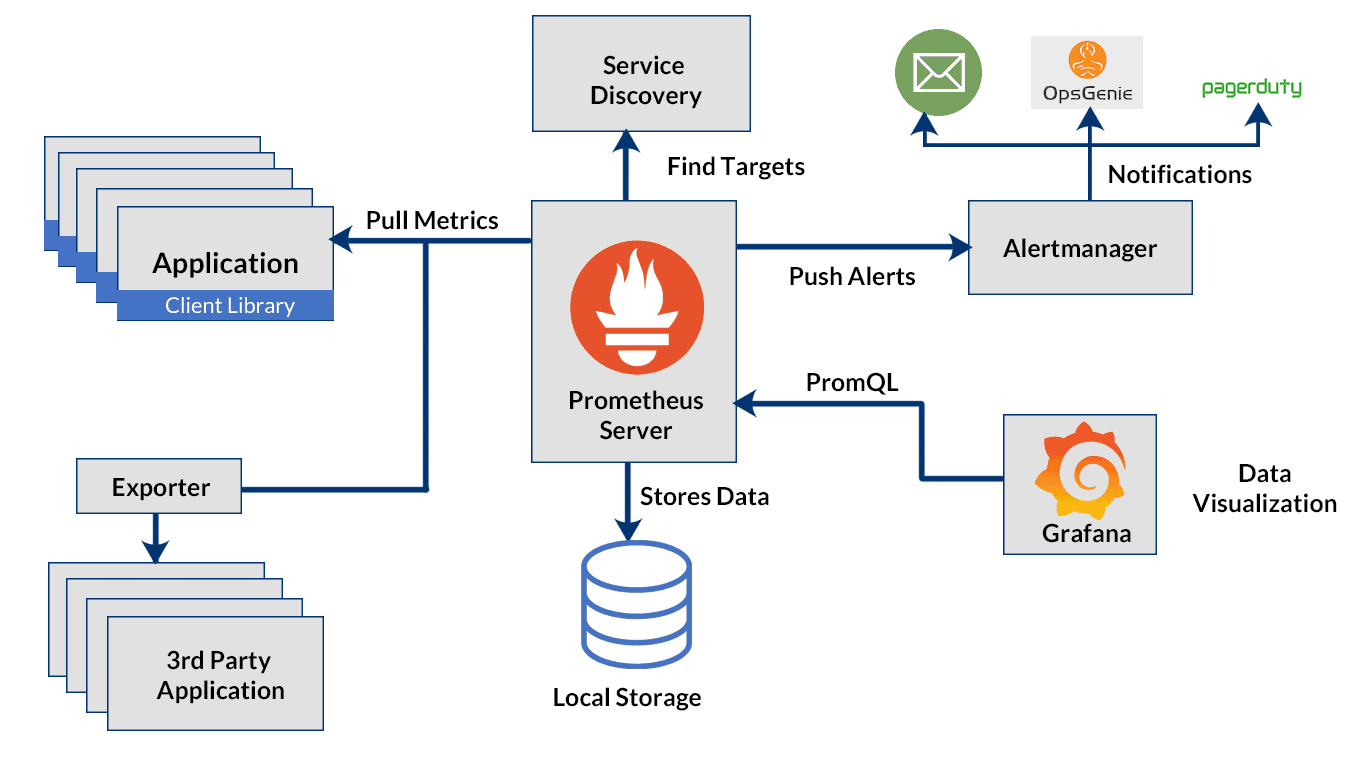
\includegraphics[scale=0.25]{prometheus-arch.png}
	\caption{معماری بخش نظارت}
	\label{fig: monitoring arch}
\end{figure} 

 
\subsection{استقرار مدل}

استقرار مدل یکی از مراحل کلیدی در فرآیند استفاده از مدل‌های یادگیری ماشین است. در این مرحله، مدل‌های آموزش‌دیده به‌صورت سرویس‌های قابل‌دسترسی برای پیش‌بینی\footnote{\lr{Inference}} به کار گرفته می‌شوند. استقرار مدل شامل مجموعه‌ای از فعالیت‌ها و فرآیندها می‌باشد که اطمینان حاصل می‌کند مدل‌ها به‌طور مؤثر و کارآمد در محیط تولید مورد استفاده قرار می‌گیرند.

اهمیت استقرار مدل در یادگیری ماشین به دلیل توانایی آن در انتقال مدل‌های آموزش‌دیده از محیط‌های توسعه به محیط‌های عملیاتی است که در آن‌ها می‌توانند ارزش واقعی ایجاد کنند. بدون استقرار مدل، تمامی تلاش‌ها و منابع صرف‌شده برای آموزش مدل‌ها بی‌فایده خواهند بود، زیرا مدل‌ها نمی‌توانند در دنیای واقعی مورد استفاده قرار گیرند. استقرار مدل امکان دسترسی سریع و کارآمد به پیش‌بینی‌های مدل را برای کاربران نهایی، برنامه‌ها و سیستم‌های دیگر فراهم می‌کند. این امر نه‌تنها به بهبود فرآیندهای تصمیم‌گیری و کارایی کسب‌وکار کمک می‌کند، بلکه از طریق نظارت مستمر و به‌روزرسانی مدل‌ها، دقت و عملکرد آن‌ها نیز حفظ می‌شود. همچنین، استقرار مدل به سازمان‌ها اجازه می‌دهد تا مدل‌ها را به‌صورت مقیاس‌پذیر و با اطمینان از کارایی بالا به کار گیرند که این خود موجب بهبود تجربیات کاربری و افزایش بهره‌وری می‌شود \cite{kubeflowforML}.

استقرار مدل‌های یادگیری ماشین به دو روش اصلی زیر انجام می‌شود: 

\begin{enumerate}
	\item
	\lr{Embedded Model Serving}:
	در استقرار جاسازی‌شده، مدل‌ها مستقیماً در برنامه اصلی تعبیه می‌شوند. این روش باعث می‌شود که مدل‌ها بالاترین عملکرد را داشته باشند و زیرساخت ساده‌تری نیاز داشته باشند، زیرا همه‌چیز در یک واحد مجتمع شده است. اما این روش نیازمند به‌روزرسانی مجدد برنامه در هر تغییر مدل است و مقیاس‌پذیری کمتری دارد، زیرا افزایش تعداد کاربران یا درخواست‌ها می‌تواند به کاهش عملکرد منجر شود. همچنین، باید تمام استراتژی‌های استقرار به‌صورت دستی پیاده‌سازی شوند که پیچیدگی بیشتری به همراه دارد \cite{kubeflowforML}.
	\item 
	\lr{Model as a Service (MaaS)}:
	در این نوع استقرار، مدل‌ها به‌عنوان سرویس‌های جداگانه ارائه می‌شوند که می‌توانند از هر برنامه‌ای در سازمان مورد استفاده قرار گیرند. این روش مزایای زیادی دارد از جمله ساده‌سازی ادغام مدل‌ها با سایر فناوری‌ها و فرآیندهای سازمانی، امکان استفاده مجدد از مدل‌ها در برنامه‌های مختلف، و پشتیبانی از دستگاه‌های کم‌قدرت که نمی‌توانند مدل‌های پیچیده را اجرا کنند. \lr{MaaS} همچنین امکان استفاده از تکنیک‌های پیشرفته مانند به‌روزرسانی مدل، تشخیص انحراف مدل و غیره را فراهم می‌کند \cite{kubeflowforML}. علاوه بر این، این روش اجازه می‌دهد که مدل‌ها و برنامه‌ها به‌طور مستقل مقیاس‌بندی شوند و می‌توانند بر روی سخت‌افزارهای مختلف مانند \lr{CPU} و \lr{GPU} اجرا شوند. اما معایبی از جمله کاهش عملکرد به دلیل وجود شبکه‌های اضافی و پیچیدگی‌های مدیریت هماهنگی زمانی بین سرویس مدل و برنامه اصلی نسبت به روش قبل دارد.
\end{enumerate}

در استقرار مدل به‌عنوان سرویس نیز، دو رویکرد اصلی وجود دارد: مدل به‌عنوان کد\footnote{\lr{Model as Code}} و مدل به‌عنوان داده\footnote{\lr{Model as Data}}. در رویکرد اول، کد مدل به‌طور مستقیم در پیاده‌سازی سرویس استفاده می‌شود. به‌عبارت‌دیگر، کد مدل بخشی از کد اصلی سرویس است که در آن قرار دارد. این روش می‌تواند برای پروژه‌های کوچک یا محیط‌های توسعه مناسب باشد، زیرا ساده‌تر و مستقیم‌تر است. اما وقتی مدل‌ها به‌روزرسانی می‌شوند، نیاز به تغییر و استقرار مجدد سرویس وجود دارد که می‌تواند زمان‌بر و پیچیده باشد. در مقابل، رویکرد مدل به‌عنوان داده از یک پیاده‌سازی عمومی استفاده می‌کند که توسط یک مدل با فرمت استاندارد مانند \lr{PFA}، \lr{ONNX} و یا فرمت اصلی \lr{TensorFlow} استفاده می‌شود. این روش مزایای زیادی دارد، از جمله استانداردسازی تبادل مدل‌ها بین سرویس‌های مختلف که قابلیت جابه‌جایی بین سیستم‌ها را فراهم می‌کند \cite{kubeflowforML}. با استفاده از این رویکرد، مدل‌ها می‌توانند به‌صورت مستقل از سرویس‌ها به‌روزرسانی شوند و نیاز به استقرار مجدد سرویس‌ها نیست. بیشتر پیاده‌سازی‌های رایج در \lr{MaaS}، مانند \lr{TFServing}، \lr{ONNX Runtime}، \lr{Triton Inference Server}، و \lr{TorchServe} از رویکرد مدل به‌عنوان داده استفاده می‌کنند و از فرمت‌های استاندارد بهره می‌برند.


\subsubsection{الزامات و انتظارات از راه‌حل‌های استقرار مدل}

استقرار مدل‌های یادگیری ماشین نیازمند درک و مدیریت جنبه‌های مختلفی است که شامل عملیات توسعه، تحلیل، آزمایش و مدیریت مدل‌ها می‌شود. این وظایف گسترده و پیچیده هستند و باید به‌صورت جامع مدیریت شوند تا مدل‌ها به‌درستی در محیط‌های عملیاتی اجرا شوند. در ادامه به بررسی مهم‌ترین الزامات و انتظارات از راه‌حل‌های استقرار مدل می‌پردازیم \cite{kubeflowforML}.

\begin{itemize}
	\item 
	انعطاف‌پذیری فریم‌ورک:
	یکی از مهم‌ترین الزامات، انعطاف‌پذیری فریم‌ورک است. راه‌حل‌های استقرار مدل باید امکان استفاده از مدل‌هایی که با فریم‌ورک‌های مختلف مانند \lr{TensorFlow}، \lr{PyTorch}، و \lr{Scikit-learn} آموزش‌دیده‌اند را فراهم کنند. این انعطاف‌پذیری به سازمان‌ها این امکان را می‌دهد که بدون نگرانی از تغییرات در فریم‌ورک‌های زیرین، از همان رابط کاربری استفاده کنند و مدل‌ها را به‌سرعت به‌روزرسانی یا تغییر دهند.
	\item 
	بهره‌گیری از بهینه‌سازهای سخت‌افزاری:
	قابلیت بهره‌گیری از بهینه‌سازهای سخت‌افزاری نظیر \lr{GPU}ها و \lr{TPU}ها یکی دیگر از الزامات مهم است. بسیاری از مدل‌های یادگیری عمیق به دلیل پیچیدگی و عمق شبکه‌های عصبی نیاز به استفاده از این بهینه‌سازها دارند. استفاده از \lr{GPU}ها و \lr{TPU}ها می‌تواند زمان پیش‌بینی را کاهش داده و کارایی مدل را بهبود بخشد.
	\item
	مقیاس‌پذیری:
	مقیاس‌پذیری یکی دیگر از الزامات اساسی است. راه‌حل‌های استقرار باید امکان مقیاس‌پذیری نمونه‌های استقرار را هم به‌صورت دستی و هم با استفاده از مقیاس‌دهنده‌های خودکار فراهم کنند. این مقیاس‌پذیری باید بدون توجه به سخت‌افزار زیرین انجام شود. همچنین، مقیاس‌دهی هر یک از اجزای چرخه کاری استنتاج باید به‌صورت جداگانه انجام شود.
	\item 
	پشتیبانی از درخواست‌های \lr{REST} یا \lr{gRPC}:
	راه‌حل‌های استقرار باید از درخواست‌های \lr{REST} یا \lr{gRPC} پشتیبانی کنند. این قابلیت‌ها امکان تعامل سریع و کارآمد با سرور مدل را فراهم می‌کنند و به انعطاف‌پذیری بیشتر در نحوه استفاده از مدل‌ها کمک می‌کنند. 
\end{itemize}

به‌منظور استقرار مدل‌های یادگیری ماشین ابزارهای متن‌باز بسیاری وجود دارند که یکی از معروف‌ترین این ابزارها \lr{KServe} می‌باشد. این ابزار یک راه‌حل پیشرفته برای استقرار و مدیریت مدل‌های یادگیری ماشین در محیط‌های تولیدی است. این ابزار به‌عنوان یک پروژه متن‌باز توسط \lr{Seldon}، \lr{Google}، \lr{Bloomberg}، و \lr{IBM} توسعه یافته است و هدف آن پر کردن خلأهای موجود در ابزارهای مهم دیگر مانند \lr{TFServing} و \lr{Seldon Core} است. \lr{KServe} با بهره‌گیری از اصول معماری \lr{Serverless} و استفاده از زیرساخت‌های کوبرنتیر و \lr{Knative}، پیچیدگی‌های مربوط به استقرار، مقیاس‌پذیری، و مدیریت مدل‌های یادگیری ماشین را کاهش می‌دهد. علاوه بر این، این ابزار از مقیاس‌پذیری دینامیک بر اساس رویدادها پشتیبانی می‌کند، که به معنای تخصیص منابع تنها در صورت نیاز است. ویژگی‌هایی مانند مقیاس به صفر\footnote{\lr{Scale to Zero}}، بهینه‌سازی استفاده از منابع و کاهش هزینه‌ها را تضمین می‌کنند. این امر همچنین به تیم‌ها اجازه می‌دهد تا تمرکز بیشتری بر توسعه و بهبود مدل‌های خود داشته باشند، بدون نگرانی درباره پیچیدگی‌های زیرساخت \cite{KServe}.
در کنار ویژگی‌های مهم یاد شده، \lr{KServe} از فریم‌ورک‌های مختلف یادگیری ماشین مانند \lr{TensorFlow}، \lr{XGBoost}،\lr{Scikit-learn} و \lr{PyTorch} پشتیبانی می‌کند. این قابلیت به کاربران اجازه می‌دهد تا مدل‌های خود را با استفاده از ابزارهای متنوع و موردعلاقه خود استقرار دهند.

از اجزای کلیدی در معماری \lr{KServe} می‌توان به دو بخش سطح سرویس و سطح داده اشاره کرد. سطح سرویس در \lr{KServe} شامل تمام پیکربندی‌ها و مدیریت‌های مربوط به سرورها و جریان‌های کاری است. این سطح با استفاده از \lr{Knative} پیاده‌سازی شده و به‌طور خاص بر ارائه سرویس‌های \lr{Serverless} تمرکز دارد. \lr{Knative} یک مجموعه از اجزا است که قابلیت‌های \lr{Serverless} را برای کوبرنتیز فراهم می‌کند و شامل ویژگی‌هایی مانند مقیاس‌پذیری خودکار، مدیریت ترافیک و استقرار آسان است. این امر به \lr{KServe} اجازه می‌دهد تا به‌طور خودکار مقیاس‌بندی کند، منابع را بر اساس نیاز تخصیص دهد و فرایندهای استقرار را ساده‌سازی کند. در مقابل، سطح داده در \lr{KServe} شامل اجزایی است که وظایف مختلفی مانند مسیریابی درخواست‌ها، بررسی سلامت سرویس‌ها، تعادل بار، و احراز هویت و مجوزدهی را بر عهده دارند. اجزای کلیدی سطح داده شامل پیش‌بینی‌کننده،‌ توضیح‌دهنده و مبدل می‌باشد. هسته اصلی سطح داده پیش‌بینی‌کننده است که مسئول اجرای مدل‌های یادگیری ماشین و ارائه پیش‌بینی‌ها می‌باشد. هر پیش‌بینی‌کننده شامل یک مدل و یک سرور مدل است که درخواست‌های ورودی را پردازش و پاسخ می‌دهد. توضیح‌دهنده یک جزء اختیاری است که توضیحات مدل را در کنار پیش‌بینی‌ها فراهم می‌کند. این توضیحات می‌توانند به کاربران کمک کنند تا درک بهتری از نتایج مدل داشته باشند و تصمیمات بهتری بگیرند. در آخر،‌ مبدل نیز مسئول مراحل پیش‌پردازش و پس‌پردازش داده‌ها است. مبدل‌ها به کاربران اجازه می‌دهند تا داده‌ها را قبل از ارسال به مدل و پس از دریافت پیش‌بینی‌ها به شکلی خاص تبدیل کنند. این کار می‌تواند شامل پاک‌سازی داده‌ها، نرمال‌سازی، و تبدیل‌های دیگر باشد \cite{KServe} (شکل ~\ref{fig: kserve dataplane}).

\begin{figure}[!t]
	\centering
	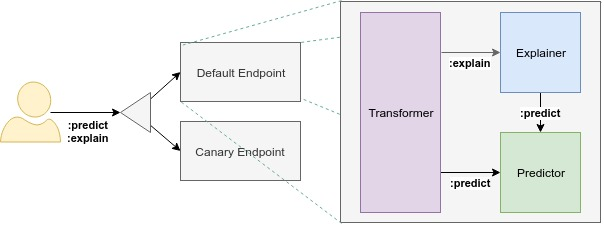
\includegraphics[scale=0.45]{kserve-dataplane.jpg}
	\caption{معماری سطح داده در \lr{KServe}}
	\label{fig: kserve dataplane}
\end{figure} 

در کنار \lr{KServe} به‌عنوان یک ابزار برای استقرار مدل به‌عنوان سرویس،‌ ابزار معروف \lr{Seldon Core} نیز وجود دارد. این پلتفرم بر پایه کوبرنتیز ساخته شده و قابلیت‌هایی مانند مسیریابی درخواست‌ها، مدیریت نسخه‌ها، نظارت بر عملکرد مدل و اندازه‌گیری متریک‌ها را فراهم می‌کند. با استفاده از \lr{Seldon Core}، می‌توان مدل‌های مختلفی ازجمله مدل‌های ساخته‌شده با \lr{TensorFlow}، \lr{PyTorch} و \lr{Scikit-learn} را به‌راحتی مستقر و مدیریت کرد. در مقابل \lr{KServe} بخشی از اکوسیستم \lr{Kubeflow} است و برای کاربرانی که از ابزارهای دیگر \lr{Kubeflow} استفاده می‌کنند، یکپارچگی بهتری ارائه می‌دهد. \lr{Seldon Core} مستقل از \lr{Kubeflow} است و می‌تواند با هر پلتفرم کوبرنتیز کار کند. همچنین، \lr{Seldon Core} از نظر پشتیبانی از الگوریتم‌های پیچیده‌تر مسیریابی درخواست و چارچوب‌های متنوع‌تر، انعطاف‌پذیری بیشتری دارد، درحالی‌که \lr{KServe} بیشتر بر سادگی و یکپارچگی با اکوسیستم \lr{Kubeflow} تمرکز دارد. در کنار این‌ها، \lr{KServe} نیز با بهره‌بردن از قابلیت \lr{Serverless} می‌تواند به مدیریت بهتر منابع کمک کند. علاوه بر این ابزار، ابزارهای \lr{TensorFlow Serving}، \lr{TorchServe} و \lr{Nvidia Triton} به‌عنوان ابزارهای روش استقرار جاسازی‌شده استفاده می‌شوند.

\subsection{جریان کاری یادگیری ماشین}
جریان‌کاری در یادگیری ماشین به‌عنوان یکی از اجزای حیاتی در مدیریت و خودکارسازی جریان‌های کاری پیچیده در حوزه‌های مختلف از جمله یادگیری ماشین و مهندسی داده، نقش مهمی ایفا می‌کند. این سیستم‌ها از گراف‌های بدون حلقه جهت‌دار برای نمایش ترتیب اجرای وظایف استفاده می‌کنند. هر مرحله از این جریان‌کاری ممکن است شامل استخراج داده، آموزش مدل یا استنتاج باشد. این سیستم‌ها نه‌تنها ترتیب اجرای وظایف را مدیریت می‌کنند، بلکه وابستگی‌های متقابل بین وظایف را نیز موردتوجه قرار می‌دهند. همچنین این ابزارها به کاربران امکان می‌دهند تا جریان‌های کاری را به‌صورت خودکار و مقیاس‌پذیر اجرا کنند. این امر به‌ویژه در محیط‌های بزرگ با داده‌های کلان اهمیت دارد.

یکی از ابزارهای مهم و معروف برای پیاده‌سازی این قسمت، \lr{Kubeflow Pipelines} می‌باشد. این ابزار یک پلتفرم قدرتمند برای مدیریت و ارکستراسیون جریان‌های کاری در زمینه یادگیری ماشین بر روی کوبرنتیز است. این پلتفرم از موتور جریان کاری \lr{Argo Workflows} استفاده می‌کند که به‌طور طبیعی بر روی کوبرنتیز قرار دارد و برای اجرای خودکار این جریان‌ها به‌کار می‌رود. \lr{Kubeflow Pipelines} با هدف ساده‌سازی فرآیند ساخت، مدیریت و اجرای خطوط لوله‌های یادگیری ماشین طراحی شده است. این پلتفرم از یک \lr{SDK} پایتون و یک زبان خاص حوزه\footnote{\lr{Domain Specific Language (DSL)}} برای تعریف جریان‌های کاری استفاده می‌کند که به کاربران این امکان را می‌دهد تا وظایف مختلف را به‌صورت برنامه‌نویسی‌شده مشخص کنند. از طریق این \lr{SDK}، کاربران می‌توانند مراحل مختلف پردازش داده، آموزش مدل، و ارزیابی را به‌صورت کد پایتون ایجاد کرده و با هم مرتبط کنند. پس از تعریف و ایجاد مراحل خط لوله، کامپایلر \lr{DSL} به‌کار می‌رود که کد پایتون را به فایل‌های \lr{YAML} استاتیک تبدیل می‌کند. این فایل‌های \lr{YAML} ساختار کامل خط لوله را به‌طور دقیق توصیف می‌کنند و به‌عنوان یک قالب استاتیک برای اجرای مراحل خط لوله در محیط کوبرنتیز استفاده می‌شوند. \lr{Pipeline Service} در مرحله بعدی، این فایل‌های \lr{YAML} را به \lr{CRD}\footnote{\lr{Custom Resource Definition}} کوبرنتیز تبدیل کرده و فرآیند اجرای خطوط لوله را مدیریت می‌کند. این فرآیند شامل ایجاد پادها و مدیریت مؤثر اجرای مراحل مختلف خطوط لوله است که توسط کنترلرهایی مانند \lr{Argo Workflow} به‌صورت خودکار انجام می‌شود. این اجزا از معماری کوبرنتیز بهره می‌برند تا اجرای خطوط لوله را بهینه و مقیاس‌پذیر کنند که این امر از اهمیت بالایی برای ایجاد و مدیریت بارهای کاری یادگیری ماشین در محیط‌های توسعه و تولیدی برخوردار است (شکل ~\ref{fig: kfp arch}).

بخش ذخیره‌سازی مؤلفه\footnote{\lr{Artifact Storage}} نقش مهمی در \lr{Kubeflow Pipelines} دارد. این بخش برای ذخیره‌سازی داده‌های تولید و مصرف شده توسط خطوط لوله استفاده می‌شود. داده‌های ذخیره شده به دو دسته اصلی تقسیم می‌شوند. دسته اول فراداده‌هایی شامل اطلاعاتی از جمله آزمایش‌ها، اجراها و معیارهای متفرقه هستند. این اطلاعات در یک پایگاه داده \lr{MySQL} ذخیره می‌شوند که امکان جستجو، مرتب‌سازی و فیلتر کردن آن‌ها را فراهم می‌آورد. دسته دوم نیز مؤلفه‌هایی شامل بسته‌های خطوط لوله حاوی کدها، فایل‌های اجرایی، یا هر نوع فایل موردنیاز برای اجرای مراحل مختلف خطوط لوله و نمودارها است. این مؤلفه‌ها در \lr{MinIO} ذخیره می‌شود. این سیستم ذخیره‌سازی به کاربران این امکان را می‌دهد تا داده‌های تولیدی و مصرفی خود را به‌طور کامل مدیریت کنند و به‌راحتی به آن‌ها دسترسی داشته باشند که این امر برای تحلیل‌های بعدی، ارزیابی‌های کیفیت و اصلاحات مدل‌ها اهمیت زیادی دارد.

\begin{figure}[t]
	\centering
	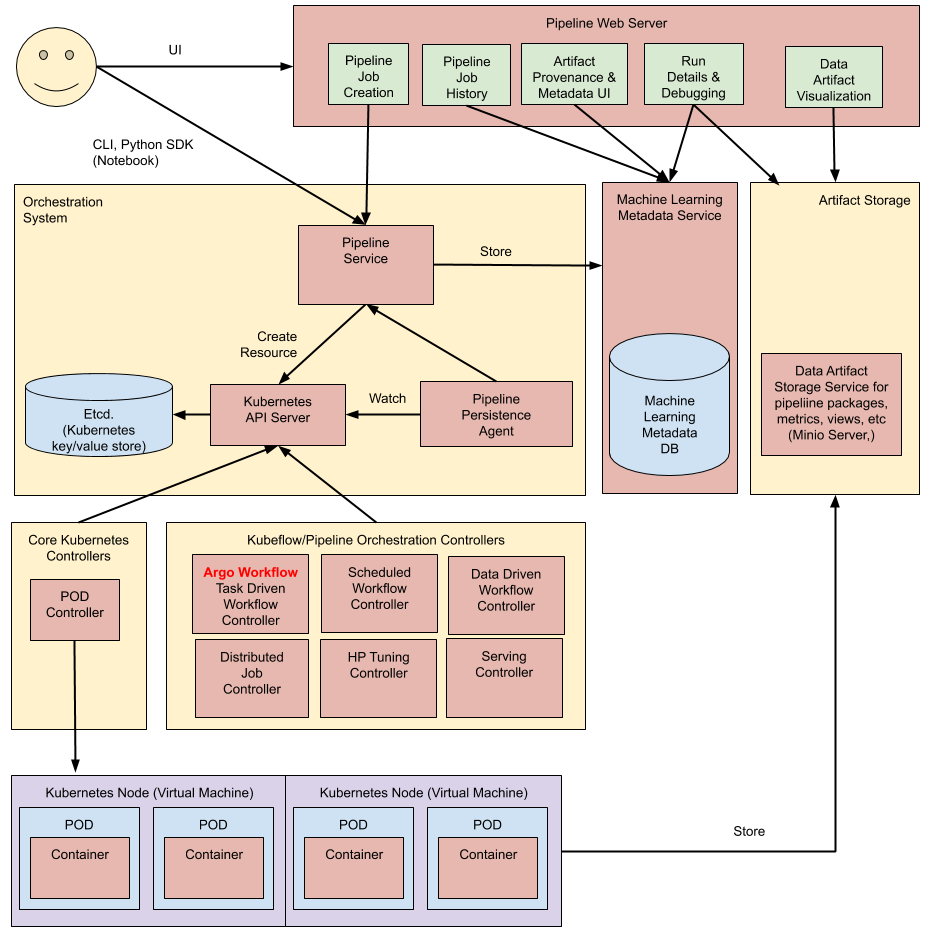
\includegraphics[scale=1.5]{kfp-arch.png}
	\caption{معماری \lr{Kubeflow Pipelines}}
	\label{fig: kfp arch}
\end{figure}

در کنار \lr{Kubeflow Pipelines}، \lr{Apache Airflow} یک ابزار متن‌باز و قابل تنظیم برای اجرای و مدیریت جریان‌های کاری است که ابتدا توسط \lr{Airbnb} توسعه داده شد و سپس توسط \lr{Apache Software Foundation} منتشر شد. \lr{Airflow} از یک معماری مبتنی بر گراف‌های بدون‌حلقه‌ی جهت‌دار استفاده می‌کند که به کاربران امکان می‌دهد تا جریان‌های کاری خود را همانند \lr{Kubeflow Pipelines} به‌صورت گرافیکی تعریف کنند. \lr{Airflow} قابلیت‌هایی مانند زمان‌بندی مراحل کاری، اجرای موازی تسک‌ها، مدیریت وظایف متکرر، مدیریت وابستگی‌ها و ارسال اعلان‌ها را فراهم می‌کند که بیشتر در زمینه‌های داده و پردازش \lr{ETL} استفاده می‌شود.

یکی از تفاوت‌های کلیدی بین این دو ابزار، سطح انتزاع و تخصص آن‌ها است. \lr{Airflow} انعطاف‌پذیری بالایی دارد و می‌تواند برای طیف گسترده‌ای از گردش کارها به‌کار رود، اما نیازمند پیکربندی و کدنویسی بیشتری است. در مقابل، \lr{Kubeflow Pipelines} با ارائه کامپوننت‌ها و توابع مخصوص به یادگیری ماشین، فرآیند ایجاد و مدیریت گردش کارهای یادگیری ماشین را ساده‌تر و مؤثرتر می‌سازد. همچنین، \lr{Kubeflow Pipelines} به‌صورت بومی بر روی کوبرنتیز اجرا می‌شود که امکان مقیاس‌پذیری بالاتری را فراهم می‌آورد، درحالی‌که \lr{Airflow} می‌تواند روی زیرساخت‌های مختلفی اجرا شود. علاوه بر این، \lr{Kubeflow Pipelines} از سیستم‌های ذخیره‌سازی برای مؤلفه‌ها و فراداده‌ها استفاده می‌کند که برای مدیریت و تحلیل اطلاعات داده‌های تولید و مصرف شده توسط خطوط لوله موردنیاز در یادگیری ماشین بسیار حیاتی است. به‌طورکلی، \lr{Kubeflow Pipelines} با امکانات و ویژگی‌های خود، بهترین گزینه برای توسعه، اجرا، و مدیریت جریان‌های کاری مرتبط با یادگیری ماشین است.


